\chapter{柔性可穿戴体-机交互接口的共享自主解码方法}

对于截肢患者和四肢瘫痪患者而言,定制化的人机交互界面在辅助机器人操控方面发挥至关重要的作用,不仅仅可以提高他们的生活自理能力,且可以在一定程度上减轻社会和家庭的护理负担。在本章节中,我们首先基于柔性拉伸/弯曲传感器网络和一个惯性传感器设计了一种可穿戴式身体-机器交互界面,通过测量使用者斜方肌和胸小肌的肌肉形变进而将其肩部运动映射为连续的二维操控指令。针对传感器数据,设计了两种数据映射模型:基于预定义规则的直接数据线性映射方式和考虑到不确定性的意图推断数据解码方法,用于将高维度的传感器观测数据映射到二维操控界面。由于不同映射模式在动态响应能力操控精准度存在区别,我们通过一个实验将用户的使用直接数据映射模式的操作表现先验知识结合到共享自治框架中,实现了两种数据解码方式的自适应切换来增强交互命令生成的整体性能。最后,我们通过一系列光标操控实验和一个虚拟电动轮椅驾驶任务验证了所提出交互界面和数据解码方法的有效性。所提出的交互界面有可能在未来集成设计到到服装中,从而实现失能人员在日常生活中对各类辅助机器人的非侵入性交互操控。

\section{研究动机}    
四肢瘫痪和上肢截肢,尤其是因交通事故、工伤、跌倒和枪伤等原因导致的,不仅对受影响者的生活质量产生巨大负面影响,还严重削弱了他们进行日常自我护理的能力。其中四肢瘫痪是指横贯性病变发生在脊髓较高水平位上,一般将第二胸椎以上的颈脊髓横贯性病变引起的截瘫称为高位截瘫。根据中国残疾人联合会数据,中国的肢体残疾人数量为2400万人左右\cite{ZhongGuoCanJiRenFuLiJiJinHuiHuoJuan600WanYuanBangFuPinKunZhiCanRenShi_GunDongXinWen_ZhongGuoZhengFuWang},其中截肢和四肢瘫痪是肢体残疾中较为严重的类型之一,他们中的大多数人最终部分或完全依赖于他们的照顾者\cite{vitorinodinizRachimeduralTraumaEpidemiology2016}。世界卫生组织已经呼吁各国积极推进辅助设备的研究,我国在2021年九月发布了《中国脊髓损伤者生存质量白皮书》意在促进脊髓损伤辅助相关研究工作的推进。根据一项调查研究表明,除了恢复运动能力外,他们的主要兴趣之一是能够控制辅助机器人或电子设备,例如电脑、轮椅、机械臂和智能假肢。这些设备将有效提高他们日常生活的独立性,并减轻家庭的照顾负担    \cite{orejuela-zapataSelfHelpDevicesQuadriplegic2019}。因此,由于他们运动能力的缺陷,通常需要定制的人机交互界面来满足不同的需求。  

如论文第一章所述,目前基于生理信号的定制化人机交互方式已得到了广泛研究。其中已有研究应用脑机接口(BCI)操控智能电动轮椅\cite{cruzSelfPacedBCICollaborative2021}、控制虚拟飞行器\cite{krygerFlightSimulationUsing2017}以及遥控操作辅助机械臂\cite{gilliniAssistiveSharedControl2021}。然而,基于生理信号的交互设备通常存在带宽低、使用者培训和练习使用周期长、计算需求高以及需要用户高度集中的问题。由于得到的传感器数据没有直接的物理意义,因此大多数该类型的交互设备只能在有限的离散命令空间中工作。最近的一项用户研究显示,四肢瘫痪患者更倾向于使用方面的可穿戴交互设备\cite{zhangUnderstandingInteractionsSmart2022}。非侵入式的可穿戴体-机交互接口通过对身体某些部位(如头部,手指,耳部肌肉等位置)的运动跟踪来执行实时感知信号获取,因此侵入性较小,已有研究正在对其成为定制化交互界面的可能性进行了研究\cite{miehlbradtDatadrivenBodyMachine2018a,zhouNonInvasiveHumanMachineInterface2022}。与捕获脑机接口捕获大脑激活电信号不同,体机交互设备通常需要捕获人体的肌肉活动。因此,在设计定制化体-机交互界面之前,首先需要明确使用者的残余活动能力。颈椎脊髓损伤的分级主要依据ASIA(美国脊髓损伤协会)制定的标准\cite{SpinalCordInjury},具体如下:

\begin{itemize}
\item A级:完全性脊髓损伤。损伤平面以下所有感觉、运动功能完全丧失,包括自主呼吸功能。患者需要终身依赖呼吸机或其他辅助设备维持生命。
\item B级:不完全性脊髓损伤。损伤平面以下存在感觉功能,但无运动功能。患者可以感知疼痛、温度等刺激,但不能进行自主运动。根据感觉功能保留的范围,B级又可分为B级-完全感觉和B级-部分感觉。
\item C级:不完全性脊髓损伤。损伤平面以下仅有一些肌肉运动的功能,无有用功能的存在。患者可以完成一些简单的动作,如移动肢体、维持姿势等,但无法进行日常生活活动或参与社会活动。
\item D级:不完全性脊髓损伤。损伤平面以下保留了部分的运动功能。患者可以完成一些日常生活活动,如行走、穿衣、进食等,但存在一定程度的障碍。根据运动功能保留的范围,D级又可分为D级-完全运动和D级-部分运动。
\item E级:正常或接近正常的脊髓功能。患者的感觉和运动功能基本正常,但可能存在一些异常的反射。这种情况通常不需要特殊治疗,患者可以恢复正常的生活和工作。
\end{itemize}

根据损伤脊椎节段不同,可以将颈脊髓损伤分为C1至C8等8个级别,其症状和有所不同。C1至C4级别为高位颈脊髓损伤,其中C1、C2级别最为严重,通常表现为颈部以下完全瘫痪、失去独立呼吸能力、行动极为有限,需要护理人员全面协助、因说话受到影响导致沟通困难。由于此类人群基本没有任何自主活动能力,无法使用辅助设备,因此不在本文的研究讨论范围内。C3,C4级别的脊髓损伤可以控制膈膜,这一级别的患者可以自主呼吸并说话。相较于高位颈脊髓损伤,如图\ref{3-fig-1}所示,在C5级别的脊髓损伤下,患者可以举起手臂或弯曲肘关节,但是可能无法控制手腕,手,躯干,双腿;可以说话但是呼吸能力较弱,需要呼吸机辅助,耐力差并需要帮助清除唾液。可以使用电动轮椅,但是需要完全的协助才能进出椅子,需要辅助设备进餐,每天需要两到六个小时的他人辅助来完成日常生活。C6级别脊神经会影响控制手腕伸展的能力,患者通常在手部,躯干和腿部出现麻痹症状,但是可以向后弯曲手腕;可以说话,呼吸较弱。可以在没有辅助的情况下上下床。C7至C8级别的患者可以控制某些手部动作,其中大部分患者可以抓取和释放物体,可以正常说话,可以活动肩膀、手臂、手,但会有些手部肌肉无知觉。
综合来看,大多数不完全性脊髓损伤四肢瘫痪患者在其肩部周围仍有剩余的主动活动能力\cite{shefflerNeuromuscularElectricalStimulation2007},这为设计体-机交互界面提供了可行性。

\begin{figure}[!t]
    \centering
    \includegraphics[width=1\textwidth]{3-fig-1.pdf}
    \caption{部分颈脊髓损伤运动感知能力分级示意图}
    \label{3-fig-1}
\end{figure}     

\section{体-机交互界面系统设计} 
已有研究使用惯性测量单元和视觉传感器来收集四肢瘫痪患者的肩部运动以控制智能轮椅\cite{thorpUpperBodyBasedPower2016d,seanez-gonzalezCursorControlKalman2014}。然而,这些系统仅能测量所附着标记或传感器位置的移动,无法选择性地捕获用户的相应肌肉激活模式,容易受到外部环境噪声的干扰。为解决这一问题,已有研究将肌肉电信号与惯性传感器结合以捕获肌肉激活活\cite{rizzoglioHybridBodyMachineInterface2020},但是该类型方法仍然需要捕获高质量的生理信号。
可穿戴式的柔性应变传感器目前成为了一种设计人机交互界面的一种新方法\cite{dongStretchableHumanMachine2020}。这类传感器通过在不显眼的方式下测量皮肤或纺织品的形变来对人体运动进行跟踪。与惯性传感器不同,柔性传感器通常不存在积分漂移的问题,因此线性度以及可重复性较好,不需要频繁校准系统。当附着在特定肌肉群的位置时,柔性传感器可以通过测量肌肉的形变进而选择性地捕捉肌肉激活模式或关节运动信息。由于柔性传感器捕获的信息具有物理意义,因此相较于生理电信号通常更可靠且可以实现实时的计算处理。目前,柔性应变传感器已被部分研究用于捕捉人体肩关节的运动学信息\cite{jinSoftSensingShirt2020,leePrintableSkinAdhesive2016,samper-escuderoEfficientMultiaxialShoulderMotion2020}或实现上身/全身姿势的运动捕捉\cite{contreras-gonzalezEfficientUpperLimb2020,ogataEstimatingMovementsHuman2019,kimDeepFullBodyMotion2019}。然而,目前大多数的相关研究都围绕使用传统的运动捕捉系统作为基准,通过同步采集大量的人体运动学数据,进而通过监督学习的方法建立回归模型将柔性传感器采集得到的数据映射到关节角度。而与这些研究不同的是,在本章中。由于人体肩部是人体上肢最复杂的部分,为了高效地采集运动数据,我们首先需要对人体肩部的骨骼肌肉模型进行分析以确定传感器的最优放置位置。此外,针对传感器数据采集过程的不确定性,需要设计高效的数据解码方法将所采集的的高维传感器数据映射到低维命令空间中。  

\subsection{人体肩部肌肉骨骼模型}
肩关节是人类全身活动度最大的关节,同时也是最不稳定的关节,它具有非常大的活动度,如:在额妆面可做屈伸运动,在矢状面可做外展内收运动,在水平面可做环绕运动和屈伸运动,在垂直方向可做内旋和外旋。。骨骼方面,肩部骨骼由肩胛骨、锁骨和肱骨组成。肩胛骨位于背部,是肩部最大的骨骼,它与锁骨和肱骨相连,形成肩关节。锁骨位于胸部上方,连接肩胛骨和肱骨,使手臂能够自由活动。肱骨是手臂最长的骨骼,连接肩关节和肘关节,使手臂能够弯曲和伸展。肌肉方面,肩部肌肉可以分为四组:(1)肩胛胸肌肉:控制肩胛骨的运动,包括斜方肌、菱形肌、肩胛提肌和前锯肌。(2)仅横跨盂肱关节的相关肌肉:包括三角肌、喙肱肌、肱二头肌和肱三头肌。(3)横跨两个或更多关节的肌肉:包括胸大肌和背阔肌。(4)不直接参与肩部功能,但是很重要的解剖标志的肌肉:包括冈上肌、冈下肌和小圆肌。这些肌肉通过肌腱和韧带与骨骼相连,协同工作,使肩部能够进行各种复杂的运动, 如抬手、转动肩膀等\cite{terryFunctionalAnatomyShoulder2000}。

所设计的交互设备通过捕获肩胛骨运动(或称肩胛胸壁关节的运动)以生成连续命令,而不是依赖肩关节角度。肩胛骨参与上升、下降、前伸、后缩、上旋和下旋等六种类型的活动自由度。由于活动范围较小无法产生足够的肌肉形变,我们在骨骼肌肉模型的分析中省略了上旋和下旋两种运动模式。这些动作主要负责上肢的升降,需要大范围的运动,不适合四肢瘫痪的人。如图\ref*{3-fig-2}所示,基于OpenSim\cite{chadwickRealTimeSimulationThreeDimensional2014}的肩关节肌肉骨骼模型仿真,我们对斜方肌和胸小肌在水平和竖直两个方向上运动的肌纤维标准化长度变化特征进行了研究。斜方肌参与肩胛骨的后缩,促使肩胛骨向脊柱方向移动,反之,胸小肌对肩胛骨施加向下的力,使其向胸部移动。在肩胛骨水平前伸和后缩过程中,斜方肌和胸小肌的标准化肌纤维长度呈现出相反的变化趋势。值得一提的是,在垂直肩胛运动过程中,斜方肌的肌肉路径TS7至TS11展现出与胸小肌路径中观察到的类似变化趋势。鉴于此,我们制定了两项柔性传感器放置准则,以便最大限度地扩增所涉及交互设备可捕获的肌肉运动动态范围。首先,所选的肌肉路径在相同的运动范围内应表现出最大的标准偏差。其次,斜方肌和胸小肌的标准化长度变化应在肩胛关节运动的同一方向上呈现出相反的趋势。由此,根据这两项准则,我们在TS7、TS8、TS9和PM3、PM4路径上放置了柔性传感器,以捕捉肩胛胸壁关节在水平方向的运动。另外,将柔性传感器放置在路径TS1、TS2、TS3和PM3、PM4上,以捕获肩胛胸壁关节在垂直方向的运动。

\begin{figure}[!t]
    \centering
    \includegraphics[width=1\textwidth]{3-fig-2.pdf}
    \caption{斜方肌和胸小肌群肌肉纤维标准化长度随肩胛胸壁关节运动的变化,其中条形图显示了每组肌肉纤维随运动变化的标准偏差。}
    \label{3-fig-2}
\end{figure}     

\subsection{硬件系统设计}如图\ref{3-fig-3}所示,所开发的交互系统重量为430克,通过聚合物锂离子电池供电,在运行时的功耗约为270mW。该系统使用了四个单轴柔性弯曲/拉伸传感器和两个双轴弯曲硅胶数字电容式柔性应变传感器(由美国Nitto Bend Technologies公司生产),各个柔性传感器通过FPC排线连接至数据同步模块,并通过I2C总线以50Hz的速率将所采集到的数据上报。单轴柔性传感器能够捕获一个方向上解耦的路径无关弯曲和拉伸位移信息,而双轴柔性传感器则可以捕获两个正交方向上的路径无关弯曲信息。为了降低传感器与身体之间的滑动对于测量精度的影响,我们于压缩衬衫内放置了硅胶防滑带,并通过3D打印外壳将软传感器固定于衬衫上。四个单轴软传感器(L1、L3、R1、R3)被放置在肌肉路径TS7、TS8、TS9和PM3、PM4区域,用于捕捉相应肌肉的活动。两个双轴软传感器(L2、R2)安装在肌肉路径TS1、TS2、TS3区域,用于捕获水平和垂直方向的肩部活动。

数据同步模块置于用户背部中央区域,图\ref{3-fig-4}给出了该模块的结构框图。该模块基于STM32F103 MCU开发并内置了UCOS III操作系统用于完成任务调度,在其PCB上内置了一个MEMS惯性传感器MPU6050(包括一个三轴加速度计和三轴陀螺仪),并通过一个I2C中继器与各个柔性传感器建立通讯。数据同步采集模块可以通过无线和有线两种方式将采集到的传感器数据上传至上位机(Intel i5 10400F 2.9Ghz)。其中,无线传输基于低功耗蓝牙,有线传输基于USB,它们以50Hz的频率同步上报当前时刻的传感器数据。最后,我们使用了一个分辨率为$3840\times2160$的27英寸显示器放置在用户前方60厘米处,以提供视觉反馈,上位机的图形化界面用于提供校准以及相关的任务指引。  

\begin{figure}[!t]
    \centering
    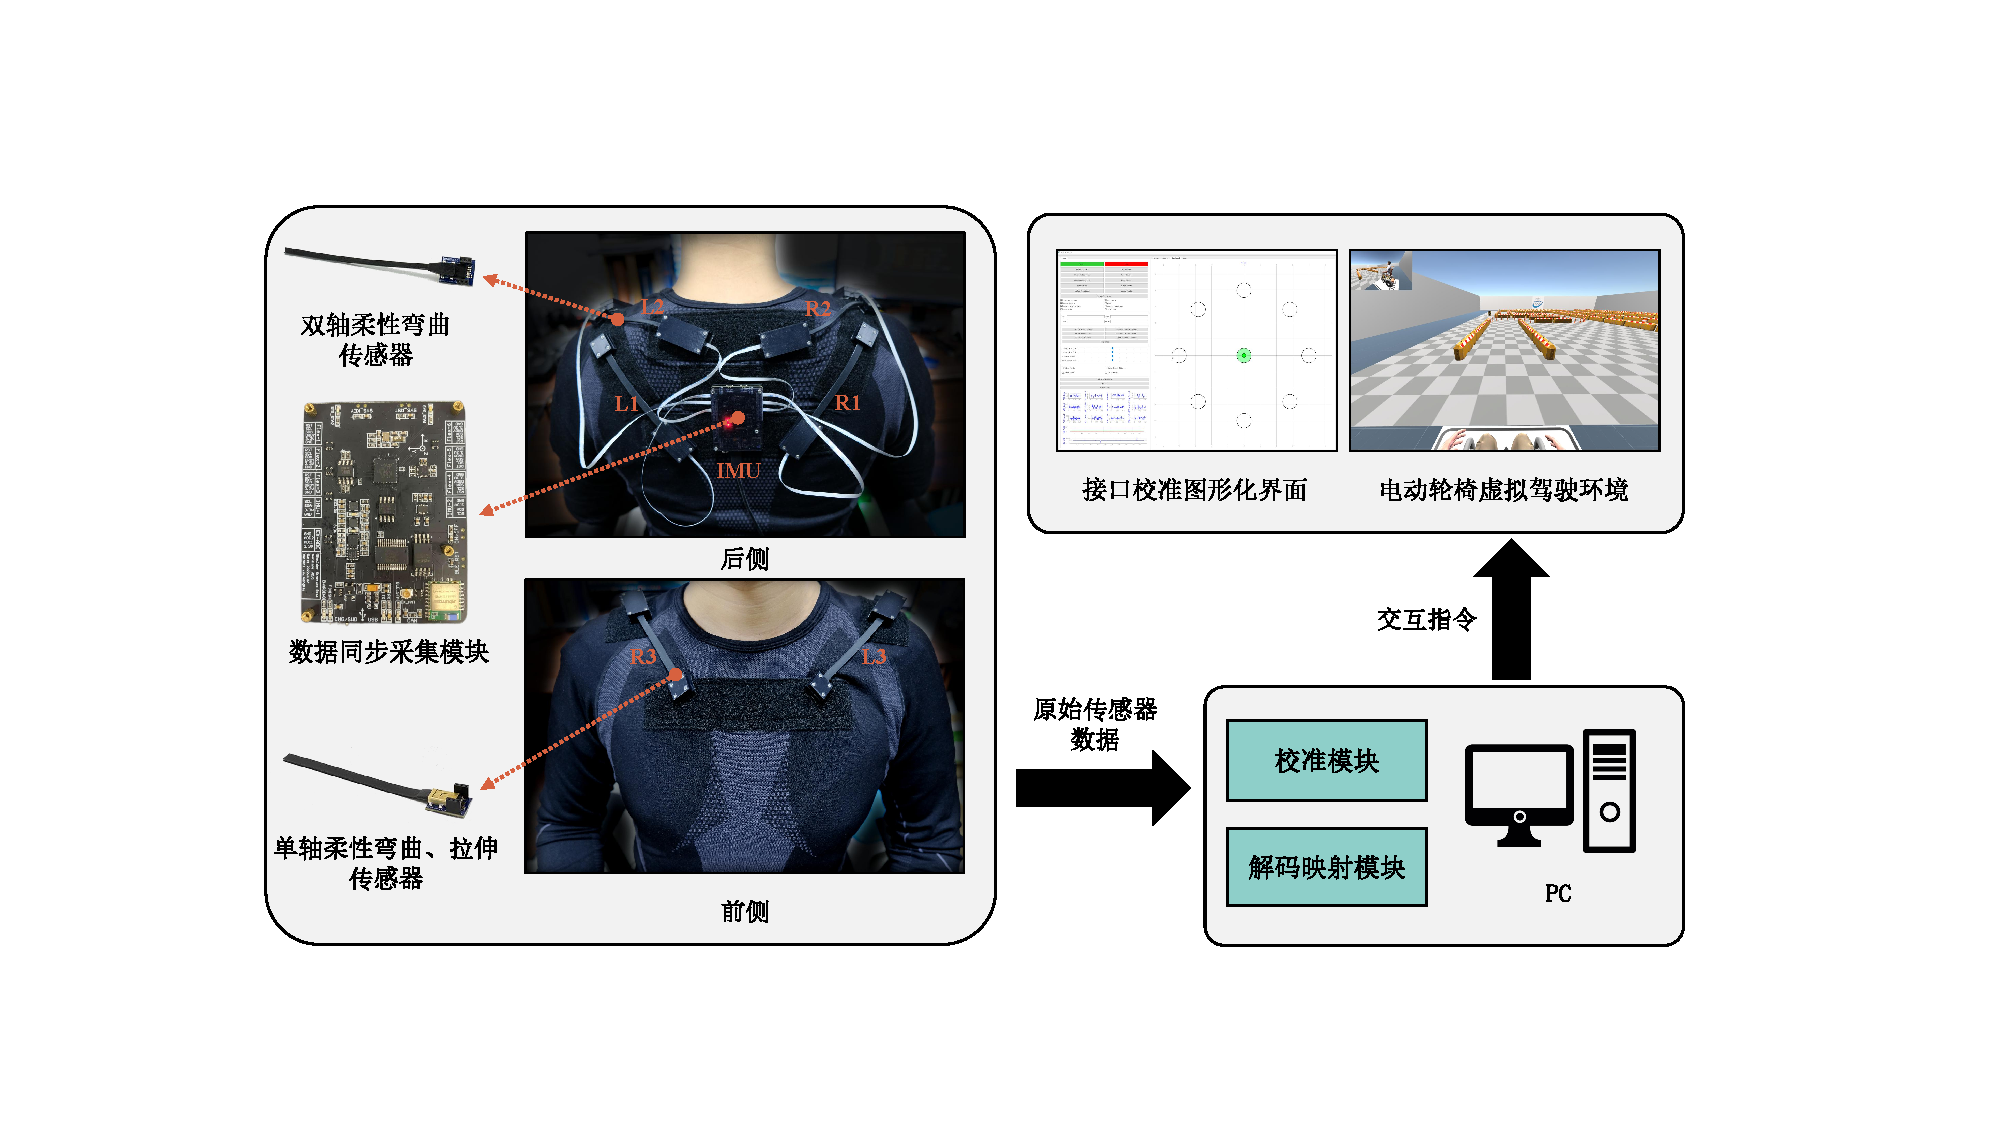
\includegraphics[width=1\textwidth]{3-Fig-3.pdf}
    \caption{所设计的体-机交互界面硬件系统结构}
    \label{3-fig-3}
\end{figure}     

\begin{figure}[!t]
    \centering
    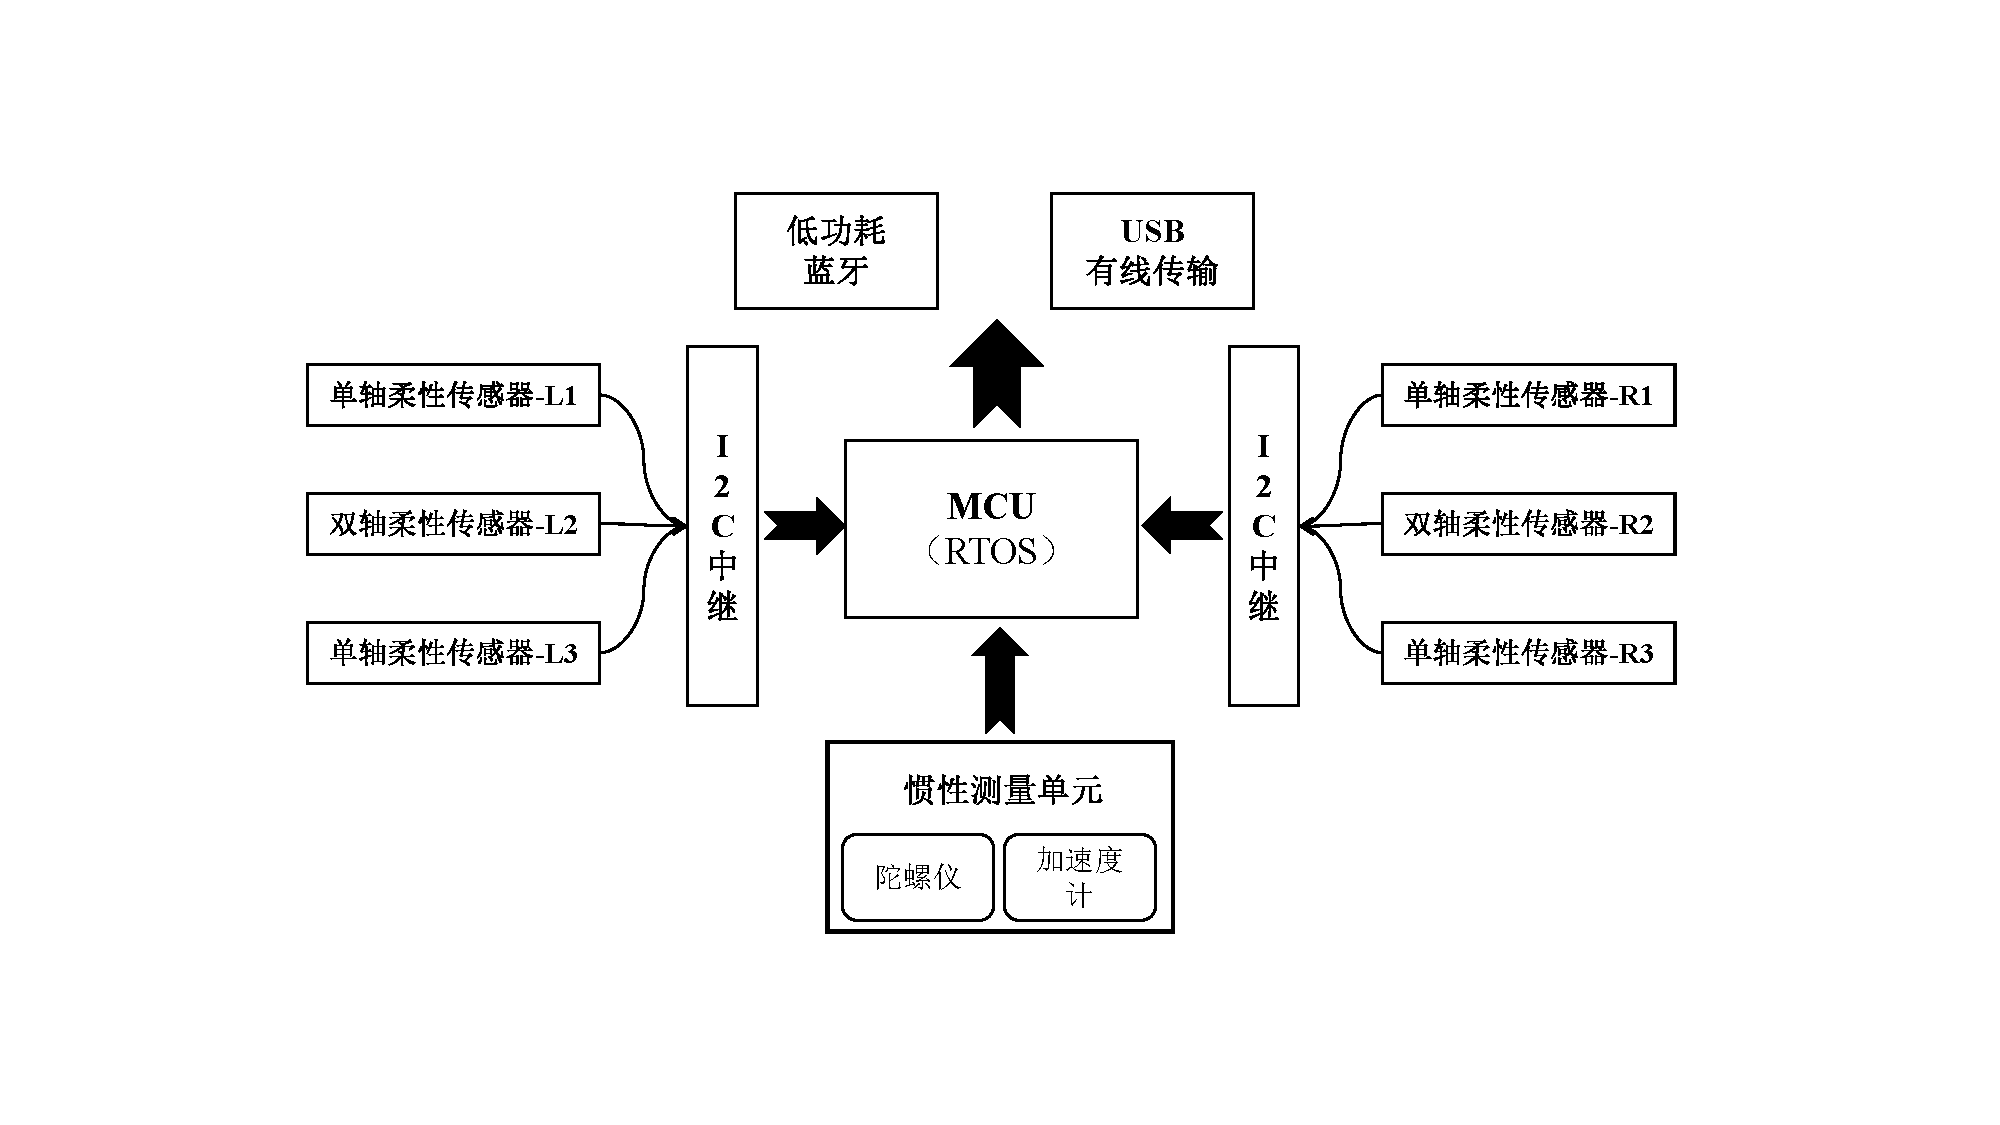
\includegraphics[width=1\textwidth]{3-Fig-4.pdf}
    \caption{数据同步采集模块结构框图}
    \label{3-fig-4}
\end{figure} 

\section{传感器数据处理与解码} 
在第二章中,我们对闭环人机交互控制外部设备的过程进行进行了分析,传感器数据处理与解码的主要目的是建立一个由观测数据到期望输出的映射函数$f(m_t)$。为此,我们利用概率图工具对交互过程进行了分析,其可建立为一个部分观测的马尔科夫决策过程(POMDP)。图
\ref{3-fig-5}给出了从$t-1$到$t+1$时刻的人机交互过程的概率图模型。其中${g_t}$表示在外部环境中用户意图实现达成的目标,${s_t} \in {\text{S}}$是外部环境的在$t$时刻的状态(可用于表示本工作中光标或轮椅的状态的状态)。${o_t}$是用户对环境的观测信息,其包括视觉、听觉、触觉、嗅觉以及对于前一时刻动作${a_{t - 1}}$的本体感觉反馈。根据当前状态${s_t}$和目标${g_t}$,根据当前对于环境的观测的信念,使用者根据内部的决策模型执行最优动作${a_t} \in \Theta $并收到奖励$R$。由于人机交互为一个人类贯序决策过程,在本工作中人类肩部的动作空间$\Theta $是高维度且连续的,因此不能用有限数量的离散量表示。因此,所设计开发的体-机交互界面可以被视为一种对于人类动作的量化表征工具,它将不可直接定义的人类物理动作${a_t}$通过观测和映射函数量化为有意义的低维命令${u_t}$。最后,${u_t}$通过环境的状态转移方程$T({s_{t+1}}|{s_{t}},{u_{t}})$进而改变外部环境的状态实现对设备的操控。

\begin{figure}[!t]
    \centering
    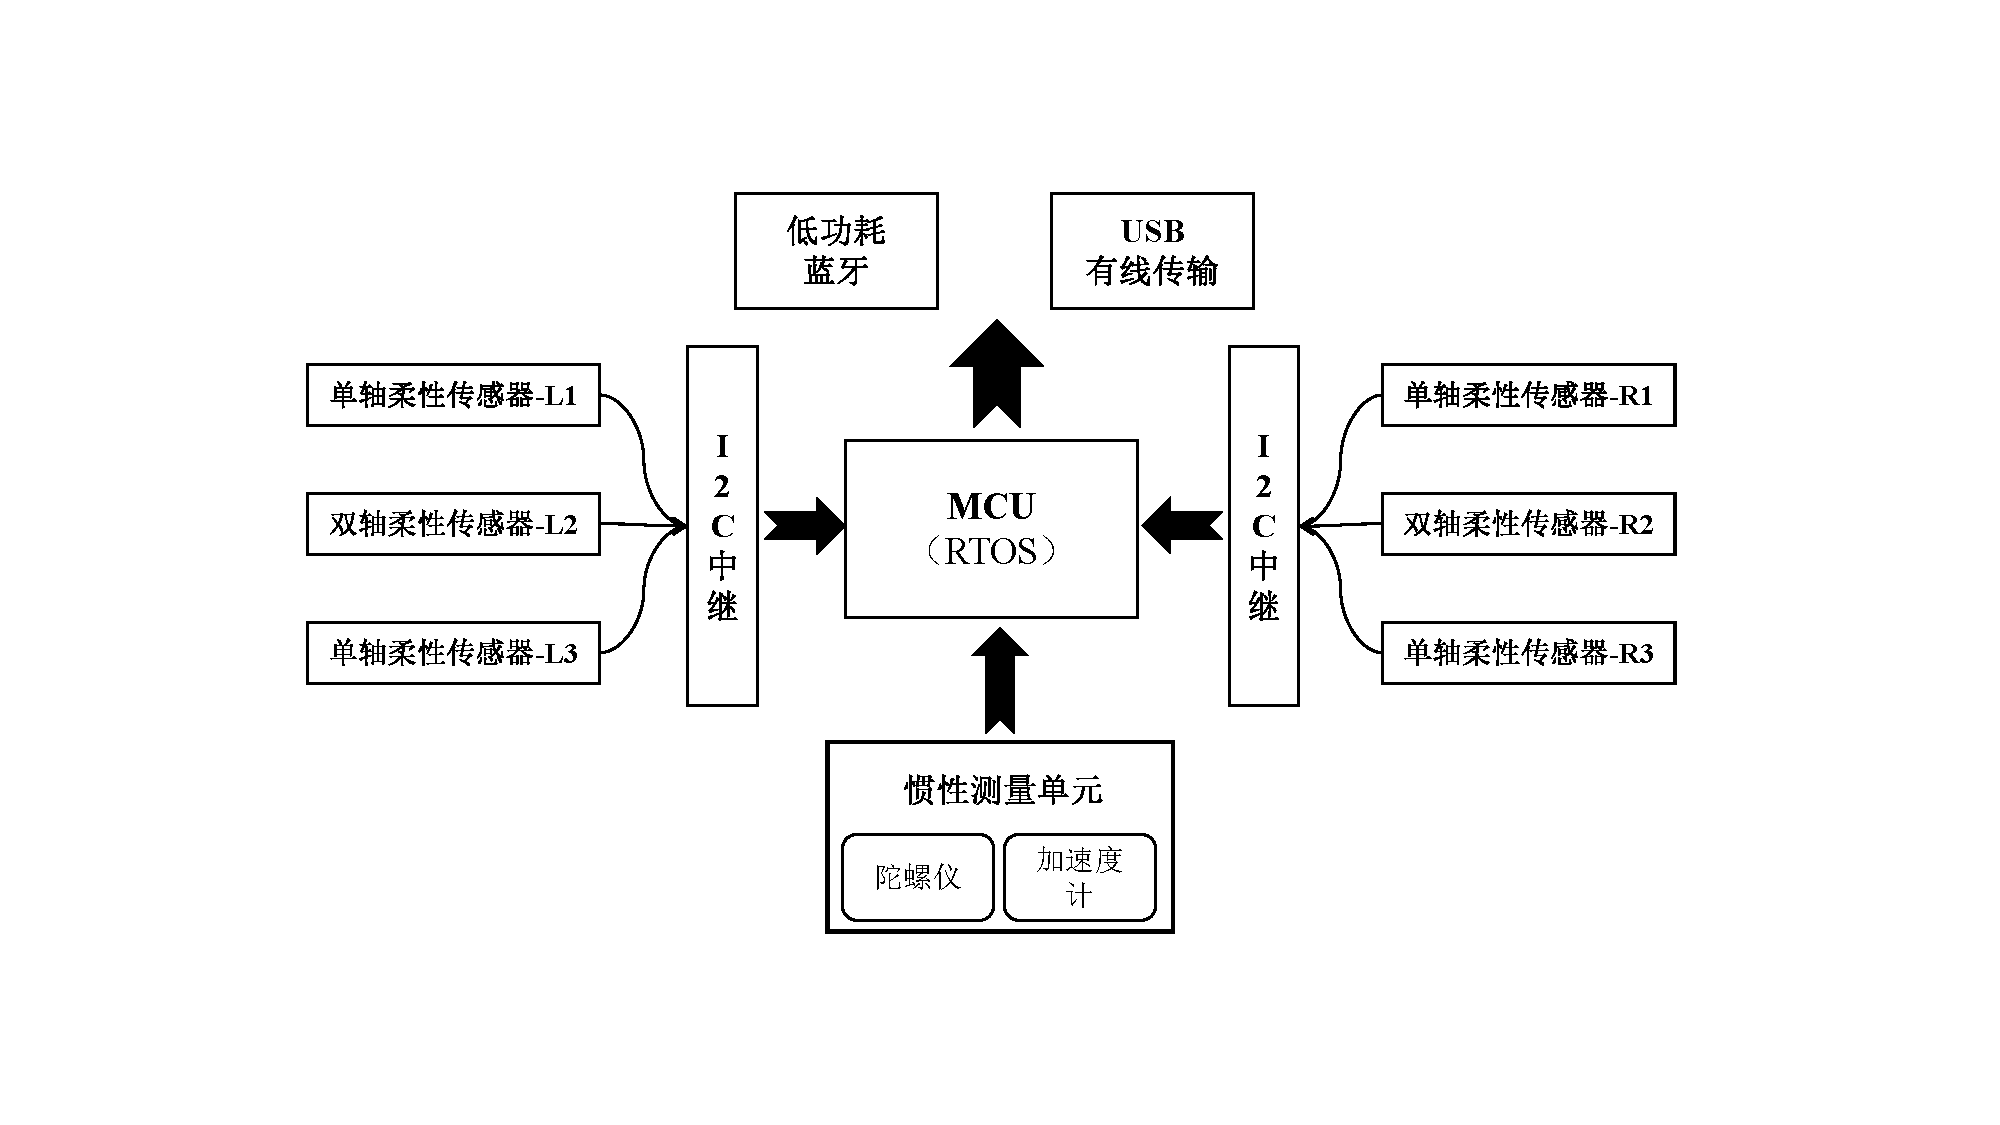
\includegraphics[width=0.4\textwidth]{3-Fig-5.pdf}
    \caption{闭环人机交互过程的概率图模型}
    \label{3-fig-5}
\end{figure} 

使用体-机交互设备时存在三个主要的不确定性来源。(1)对用户当前状态观察不充分而存在的不确定性;(2)由于用户内部建立的环境动态模型与现实世界不匹配而导致的决策不确定性;(3)由于使用者身体机能限制导致的动作执行不确定性。(4)传感器的测量噪声。由于涉及到多项不确定性来源导致难以分析,我们首先假设用户对于环境的观测是充分的并且可以准确地获取环境状态,则可认为${o_t}{\text{ = }}{{\text{s}}_t}$。此外,随着时间的推移,使用者可以通过练习了解真实的世界动态$T({s_t}|{s_{t - 1}},{u_{t - 1}})$。因此,在本章研究中我们认为不确定性只存在于使用者的动作和传感器的观测中,尽管柔性传感器测量中固有噪声相较于惯性传感器与生理信号传感器大大降低,但是体-机交互界面和用户身体在特定位置潜在的随机滑动仍然会引起不确定性。其中人类动作的不确定性已被广泛研究\cite{churchlandCentralSourceMovement2006,vanbeersRoleExecutionNoise2004, desantisGuidingFunctionalReorganization2020a}。受Gopinath等人对与防止使用者意外交互界面操作的研究\cite{gopinathCustomizedHandlingUnintended2021}的启发,我们认为预期操作$a_t$与结果操作之间的偏差是不可忽略的。对于运动障碍人士来说,固有的身体限制会增加出现动作偏差的可能性。根据用户意图提供命令至关重要,而不是仅仅依赖于传感系统的测量值,因此我们开发了两种方法分别实现了映射函数$f(m_t)$将观测信息解码为操控指令。  

\subsection{基于确定性规则映射的数据解码}
将数据从传感系统直接映射到命令空间代表了一类端到端人机交互方法,其中传感器信号直接用于线性或非线性函数的命令生成,无需考虑系统中存在的不确定性。图\ref{3-fig-6}的给出了基于确定性规则映射的数据解码方法的概率图模型,其中${m_t}$是在每个时间步长获得的传感系统的观测值。${{u}_t} = f({{m}_t})$是由线性映射函数$f$映射的控制命令。

\begin{figure}[!t]
    \centering
    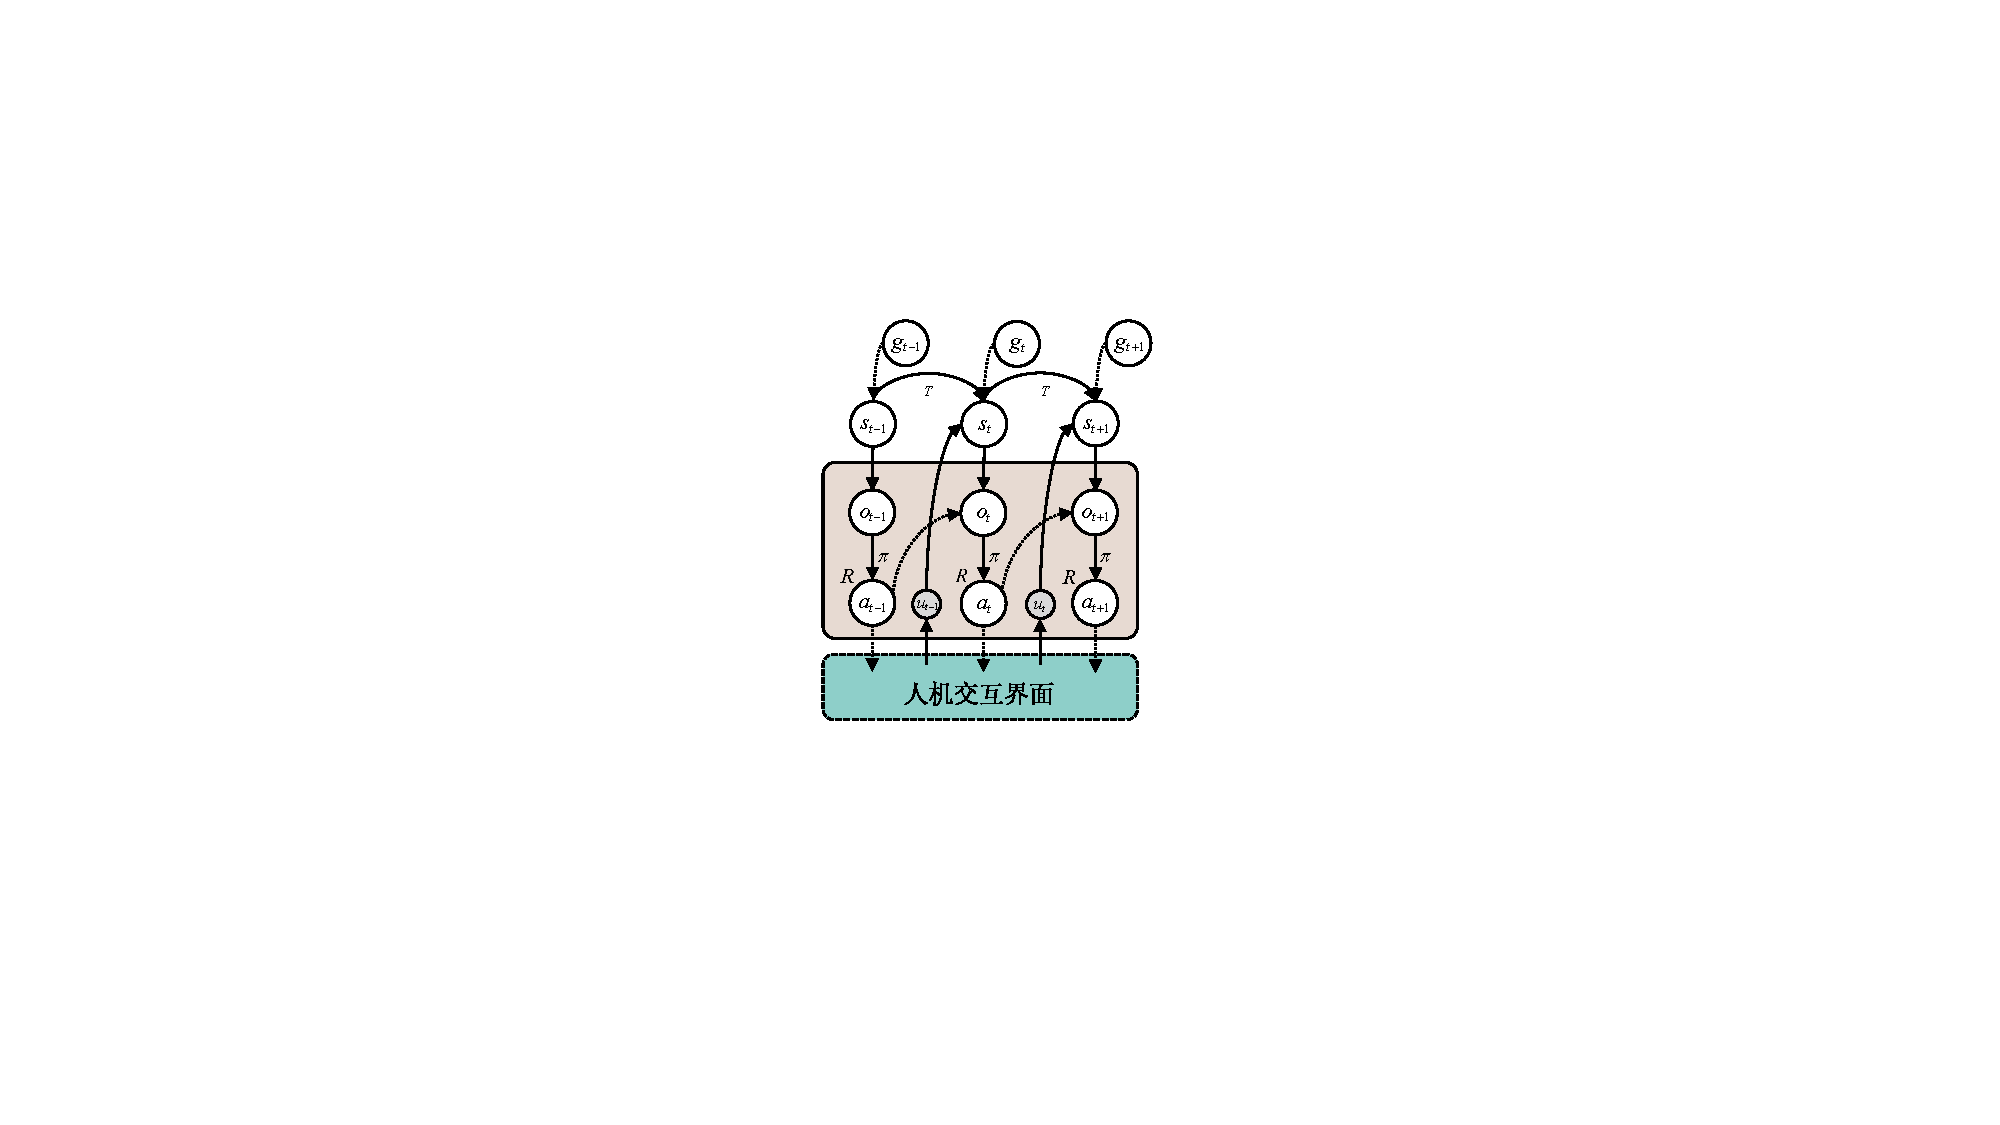
\includegraphics[width=0.4\textwidth]{3-Fig-6.pdf}
    \caption{基于确定性规则映射的数据解码方法的概率图模型}
    \label{3-fig-6}
\end{figure} 

\subsubsection{映射规则设计}
在相关研究中,主成分分析(PCA)方法通常用于将体-机交互界面的高维数据映射到低维操作命令\cite{casadioBodyMachineInterface2011,seanez-gonzalezStaticDynamicDecoding2017}。然而,基于PCA的映射模型对于用户来说往往难以将其和自身运动建立起一个清晰和直观的关系(例如光标移动方向和身体运动趋势不一致),导致用户需要大量的时间才能熟练使用它。为了解决这个问题,如图\ref{3-fig-7}所示,我们设计了一种基于规则的数据映射解码方式,将高维水平肩部运动映射到二维命令空间。其中,肩胛胸壁关节进行前伸运动生成的命令位于象限 \uppercase\expandafter{\romannumeral1}、\uppercase\expandafter{\romannumeral2}内,肩部后缩运动生成的命令位于象限\uppercase\expandafter{\romannumeral3}、\uppercase\expandafter{\romannumeral4}内。低维度的映射函数输出向量${p_t} = {[{x_t},{y_t}]^T}$和操控命令输出$u_t^{DCM}$的计算方式如下

\begin{figure}[!t]
    \centering
    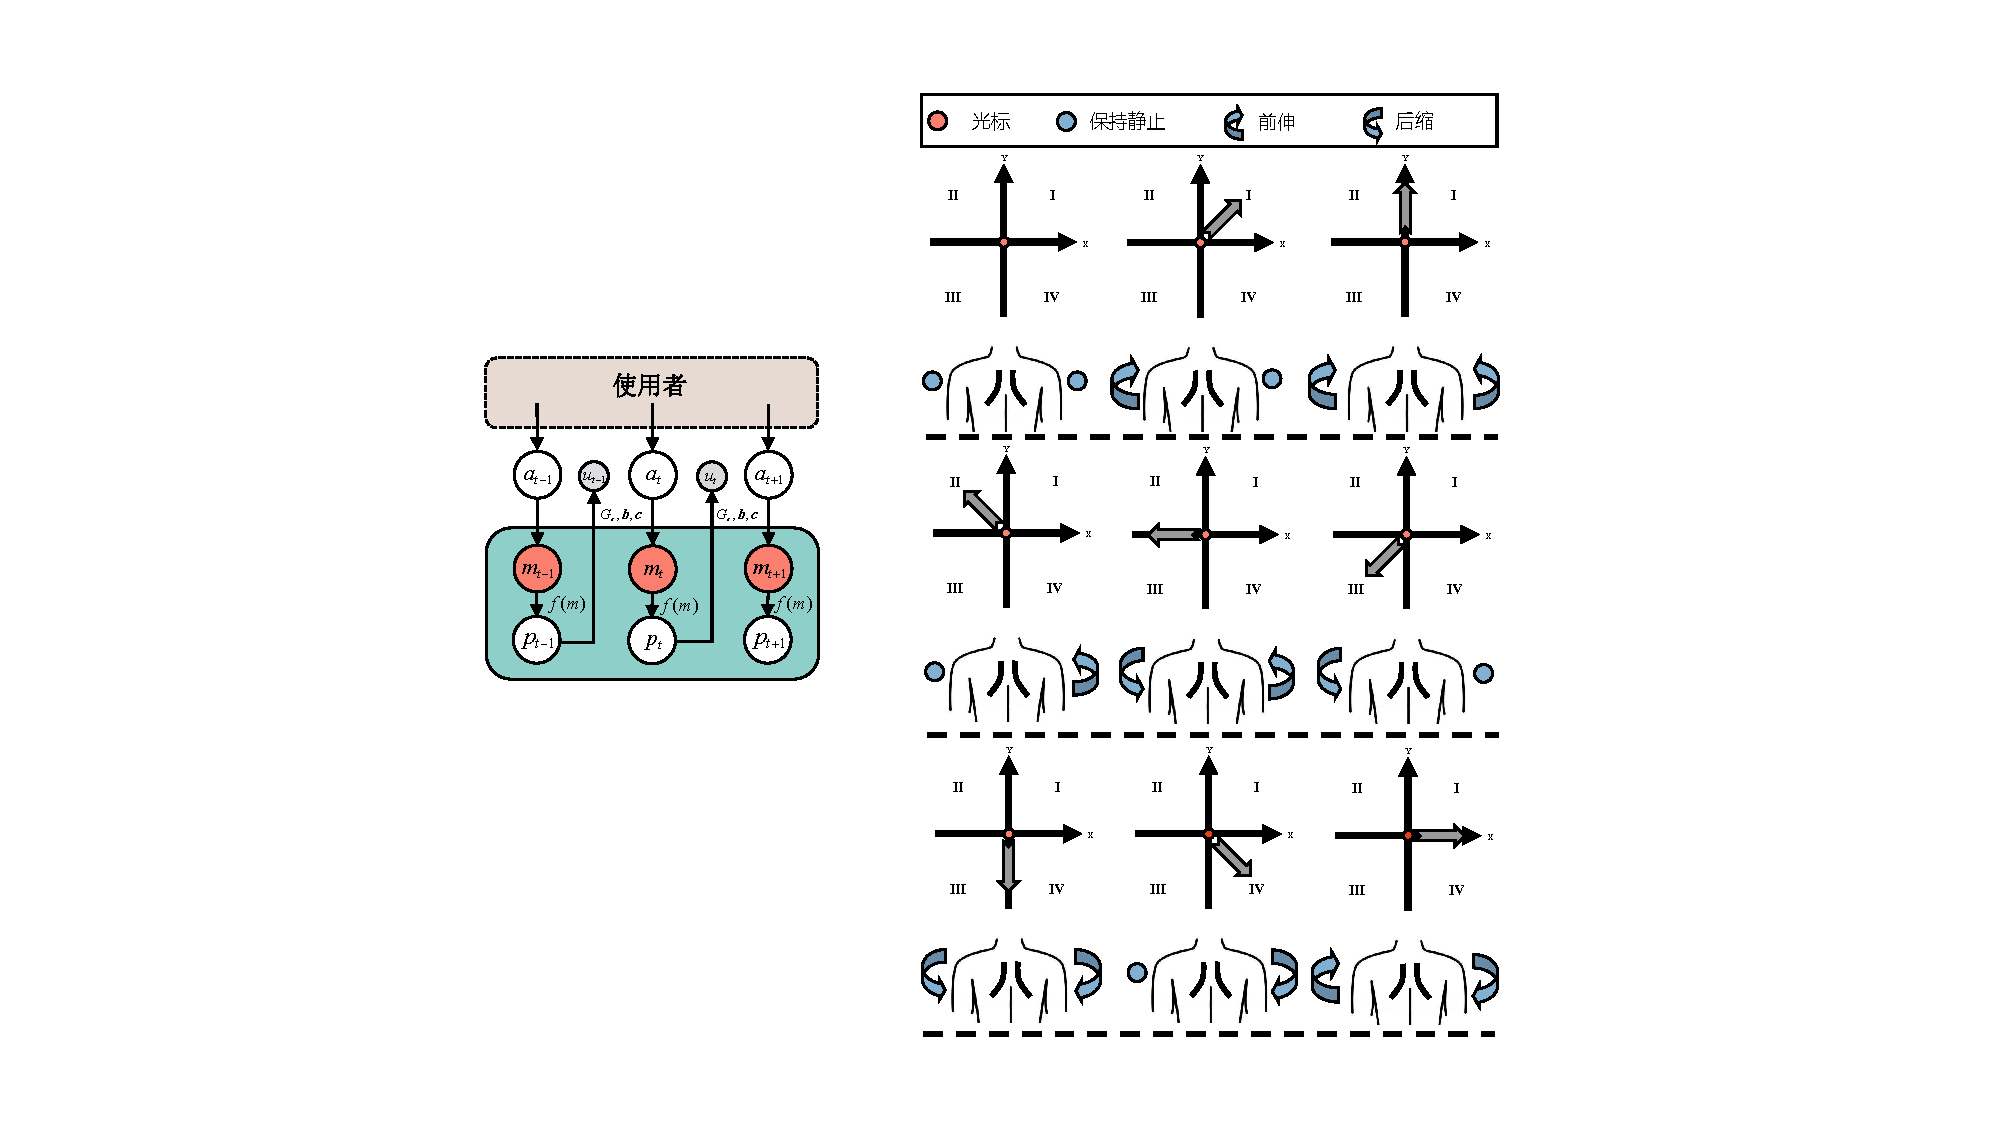
\includegraphics[width=0.7\textwidth]{3-Fig-7.pdf}
    \caption{基于确定性规则映射的数据解码方法动作与光标动作关系}
    \label{3-fig-7}
\end{figure} 

\begin{equation}
\label{eq1}
{p_t} = {\kern 1pt} \boldsymbol{{F}} \cdot \boldsymbol{{P}} \cdot {m_t}
\end{equation}   

\begin{equation}
\label{eq2}
u_t^{DCM} \triangleq {G_d}\left( {{p_t} - b} \right) \odot c
\end{equation}   

其中在$t$时刻的观测${m_t} = {[m_t^{(L1)},m_t^{(L3)},m_t^{(R1)},m_t^{(R3)}]^T}$是柔性传感器L1、L3、R1和R3测量的拉伸位移形变量。常数${G_d}$用于调整生成的命令的增益,$b\in {\mathbb{R}^{2 \times 1}}$和$c \in {\mathbb{R}^{2 \times 1}}$分别代表了零位置校准向量和尺度缩放校准向量,这两个向量在校准程序中获得。矩阵$\boldsymbol{P} \in {\mathbb{R}^{4 \times 2}}$是映射规则矩阵,$\boldsymbol{F} \in {\mathbb{R}^{2 \times 2}}$是单位旋转矩阵,它将$p_t$逆时针旋转$\pi /4$。最后,我们将左侧或右侧放置在胸小肌和斜方肌的两个柔性应变传感器的观测值之差作为命令,因此可以得到基于确定性规则的观测映射矩阵:

\[{\boldsymbol{F}} \cdot {\boldsymbol{P}} = \frac{{\sqrt 2 }}{2}\left[ {\begin{array}{*{20}{c}}
{\begin{array}{*{20}{c}}
1&{ - 1}  \\  
1&1 
\end{array}}&{\begin{array}{*{20}{c}}
{ - 1}&1  \\  
{ - 1}&{ - 1} 
\end{array}} 
\end{array}} \right]\]   

\subsubsection{校准过程}
基于确定性规则映射的数据解码的校准环节包括两个阶段。首先,我们要求参与者佩戴者以舒适放松的姿势静坐10秒钟,记录所用软传感器的拉伸数据,然后按照下式计算零点校准向量$b$:

\begin{equation}
\label{eq10}
b = \frac{1}{T}{\left[ {\sum\nolimits_{i = 1}^T {{x_i}} ,\sum\nolimits_{i = 1}^T {{y_i}} } \right]^T}
\end{equation}    

其中$T$是在10秒内记录数据的数量,${x_t}{\text{ = }}m_t^{({\text{L}}1)} - m_t^{({\text{L}}3)}$、${y_t}{\text{ = }}m_t^{({\text{R}}1)} - m_t^{({\text{R}}3)}$分别是使用者左肩和右肩位于胸小肌和斜方肌柔性传感器拉伸形变量的差值。在校准过程的第二阶段,参与者被要求尽可能最大幅度重复地前后移动左右肩膀10秒,在后期数据处理中通过使用峰值检测算法捕获记录的校准数据的极值点,用于计算缩放校准向量$c = {[{s_x},{s_y}]^T}$,其中${s_x}$和${s_y}$是缩放因子,计算公式为

\begin{equation}
\label{eq11}
{s_x} = \left \{  \begin{gathered}
    \frac{{\sum\nolimits_{i = 1}^{T_x^ + } {X_i^ + } }}{{T_x^ + }},{x_t} > 0 \hfill  \\ 
    \frac{{\sum\nolimits_{i = 1}^{T_x^ - } {X_i^ - } }}{{T_x^ - }},{x_t} < 0 \hfill  \\  
  \end{gathered}  \right.{\text{, }}{s_y} = \left \{  \begin{gathered}
    \frac{{\sum\nolimits_{i = 1}^{T_y^ + } {Y_i^ + } }}{{T_y^ + }},{y_t} > 0 \hfill  \\ 
    \frac{{\sum\nolimits_{i = 1}^{T_y^ - } {Y_i^ - } }}{{T_y^ - }},{y_t} < 0 \hfill  \\  
  \end{gathered}  \right.
\end{equation}    

其中$X_i^ + ,X_i^ - $和$Y_i^ + ,Y_i^ - $分别是第二阶段校准数据中的正峰值和负峰值。完成校准环节后,使用者自由使用身体探索光标的控制,并且手动调整它们认为最佳的增益$G_d$。 

\subsection{基于不确定性意图推理的数据解码}由于基于规则的直接映射数据解码不考虑系统中的任何不确定性因素,根据之前的分析这显然是不合理的。因此,我们进一步地将使用者使用体-机交互设备中的不确定性引入系统进行分析。在这样的框架下,我们认为用户意图产生的交互指令是不可观测的隐状态。

\begin{figure}[!t]
    \centering
    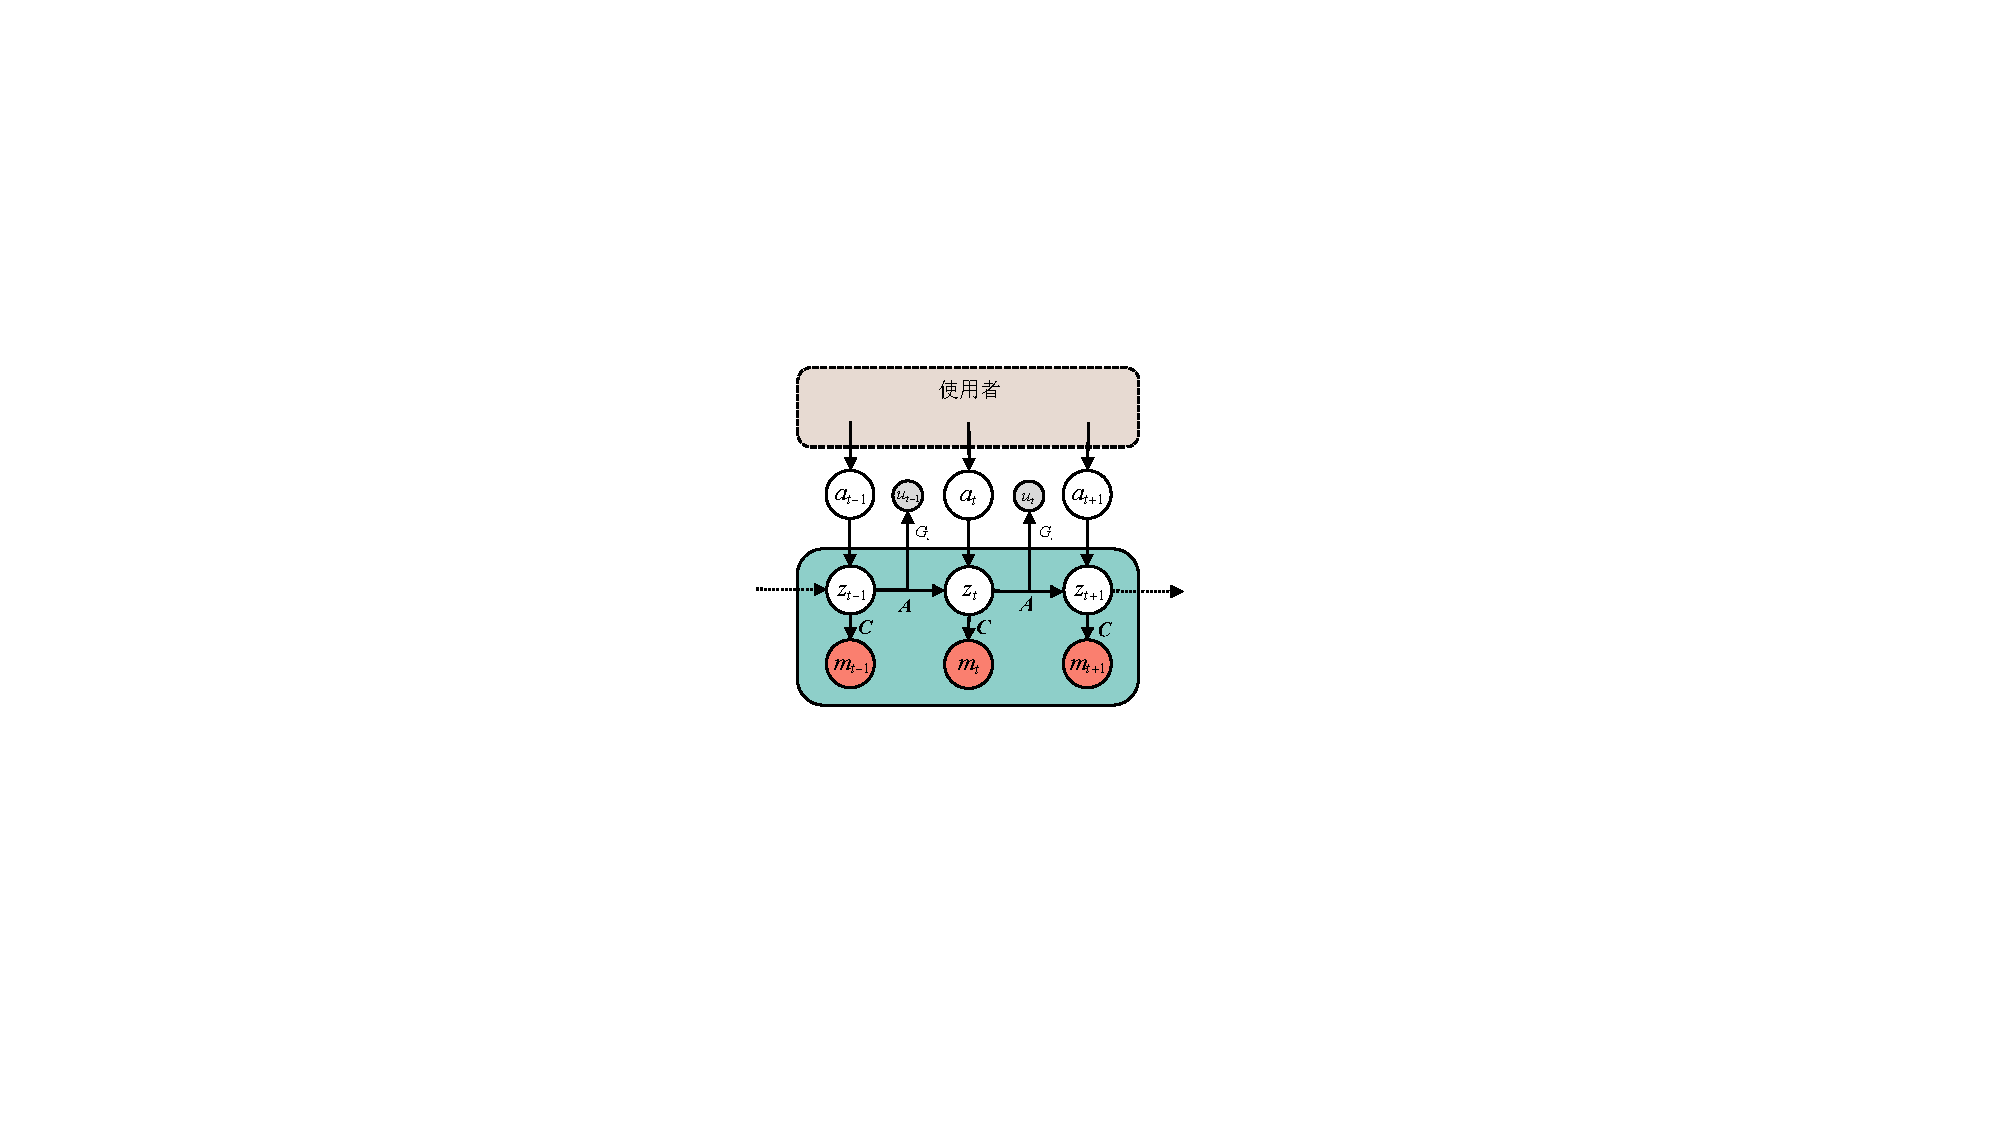
\includegraphics[width=0.52\textwidth]{3-Fig-8.pdf}
    \caption{基于不确定性意图推理的数据解码方法的概率图模型}
    \label{3-fig-6}
\end{figure} 

\subsubsection{意图推理的概率模型}
图3(A)给出了基于不确定性意图推理的数据解码方式的概率图模型给出,相较于基于规则的数据映射,其在${a_t}$和${m_t}$之间添加了不可观测的潜在变量${z_t} \in \Phi $用于表示使用者的意图,其中$\Phi$是潜在命令空间,用于表示用户可能期望发出的所有命令,在本任务中被定义为一个连续的二维平面。具体来说,意图${z_t}$表示用户在当前状态${s_t}$和目标 ${g_t}$的信念下期望生成的操控命令,则交互命令输出可以由下式定义。

\begin{equation}
\label{eq3}
u_t^{UII} \triangleq {G_i} \cdot {\hat z_t}
\end{equation}    

其中$G_i$是比例因子,在校准阶段由使用者手动调整。对于在$t$时刻的潜在用户意图${\hat z_t}$,其推理依赖于最大化后验概率$p({z_t}|{m_{1:t}})$的期望,其中$m_{1:t} \in {\mathbb{R}^{N}}$是所设计体-机交互界面传感器的观测值,由于在设计当中使用了多组柔性传感器以及一个惯性传感器,其信息往往是冗余的,需要选择使用。在这里$N$代表了用于推理的传感器配置的维度,由于我们无法直接建立观测到意图的映射关系,因此其由一个消融实验来确定。在这项工作中,为了方便计算,我们假设用户的在$t$时刻意图的操控命令与$t+1$时刻的命令之间的关系是线性的,此外假设观测数据到意图之间的映射函数$f(m_t)$也是线性的。其中相邻两个时刻的意图指令之间和传感器测量与当前意图指令之间的不确定性是服从高斯分布的,当其满足马尔科夫齐次性假设和观测独立性假设时,该模型可以表示为:

\begin{equation}
\label{eq4}
p({z_t}|{z_{t - 1}}) = \mathcal{N}({\boldsymbol{A}}{z_{t - 1}},{{\boldsymbol{Q}}_t})
\end{equation}   

\begin{equation}
\label{eq5}
p({m_t}|{z_t}) = \mathcal{N}({\boldsymbol{C}}{z_t},{{\boldsymbol{W}}_t})
\end{equation}    

其中$p({z_t}|{z_{t - 1}})$为状态转移条件概率,$p({m_t}|{z_t})$为观测条件概率。${z_t} = [{p_x}(t),{p_y}(t),{v_x}(t),{v_y}(t)]$是使用者潜在命令在时间$t$的状态,在本任务重具体表现为一个在二维空间中移动的点(光标)。${\boldsymbol{A}} \in {\mathbb{R}^{4 \times 4}}$是连续时间步之间潜在命令的先验动力学状态转移矩阵,${\boldsymbol{C}} \in {\mathbb{R}^{N \times 4}}$是传感器观测与当前用户意图命令之间的观测矩阵。${{\boldsymbol{Q}}_t} \in {\mathbb{R}^{4 \times 4}}$和${{\boldsymbol{W}}_t} \in {\mathbb{R}^{N \times N}}$分别表示了使用者的潜在意图命令在进行状态转移时的不确定性以及交互界面观测的不确定性。基于以上假设,对于使用者的意图推理过程可以看做一个状态估计问题,其最优估计可以通过卡尔曼滤波框架进行求解。其中,我们将状态转移动力学矩阵${\boldsymbol{A}}$定义为:

\begin{equation}
\boldsymbol{A} = 
\begin{bmatrix}{}
1&0&{\Delta t}&0  \\  
0&1&0&{\Delta t}  \\  
0&0&1&0  \\  
0&0&0&1 
\end{bmatrix}
\end{equation} 

其中$\Delta t$是离散系统的时间步长,观测矩阵${\boldsymbol{C}}$和状态转移不确定性协方差矩阵${{\boldsymbol{Q}}_t}$以及观测不确定性协方差矩阵${{\boldsymbol{W}}_t}$以及可以根据意图推理校准环节采集得到的训练数据计算得出。


\subsubsection{概率模型的参数估计}基于意图推理的数据解码方首先需要通过一组运动想象任务进行数据采集,该任务目前通常被用于 脑机接口神经解码数据采集的过程\cite{malikEfficientDecodingSteadyState2011,brandmanRapidCalibrationIntracortical2018a},近年来已应用于体-机交互界面数据解码\cite{seanez-gonzalezCursorControlKalman2014,seanez-gonzalezStaticDynamicDecoding2017}。在训练过程中,我们要求受试对象跟随一个在屏幕上直径为0.8厘米的红色光标,该光标在任务空间中沿着一条10厘米的直线从屏幕中心按照逆时针的顺序朝着八个方向移动。其中该红色光标的移动根据式\ref{eq3-9}所定义的微分方程进行移动\cite{seanez-gonzalezStaticDynamicDecoding2017},$x(t)$和$y(t)$分别代表了光标在显示器上的位置,$x_0$和$x_f$分别为光标的起点和终点位置,$\tau$为时间常数用于控制光标的运动速度。运动想象任务是开环的,这意味着我们不会向用户提供当前其当前使用交互界面生成的命令的任何反馈信息。受试对象需要完成三次独立的数据采集任务,期间我们记录红色目标光标移动的数据(位置和速度)和体机交互界面所采集的传感器原始数据。

\begin{equation}
    \begin{aligned}
    & x(t)=x_0+\left(x_0-x_f\right)\left(15 \tau^4-6 \tau^5-10 \tau^3\right) \\
    & y(t)=y_0+\left(y_0-y_f\right)\left(15 \tau^4-6 \tau^5-10 \tau^3\right)
    \end{aligned}
    \label{eq3-9}
\end{equation}

观测矩阵${\boldsymbol{C}}$通过运动想象务中所采集的训练数据的最大似然估计来获得,计算方式如下:

\begin{equation}
\boldsymbol{C} = YX^T(XX^T)^{-1}
\end{equation}
状态转移不确定性协方差矩阵${{\boldsymbol{Q}}_t}$和表示观测不确定性的协方差矩阵${{\boldsymbol{W}}_t}$可以通过类似的方法计算得到,计算方法如下:
\begin{equation}
{\boldsymbol{Q}}_t = \frac{1}{T-1}(X_2 - AX_1)(X_2 - AX_1)^T
\end{equation}

\begin{equation}
{\boldsymbol{W}}_t = \frac{1}{T}(Y - CX)(Y - CX)^T
\end{equation}
其中,$Y$和$X$矩阵分别是由运动想象任务记录的的体-机交互界面的传感器测量和相应的屏幕中的指引光标位置数据组成的。数据矩阵$X_1\triangleq X_{1:end-1}$和$X_2\triangleq X_{2:end-1}$,$T$为采集的训练数据量。

完成运动想象训练的数据采集和参数更新后,使用者可以通过在任务空间中自由地移动控制光标控件来手动调整增益${G_i}$。当用户感觉当前训练的意图推理模型不能很好地工作时,我们将数据采集和训练重新进行直至使用者可以使用他们的肩胛骨控制光标运动。至于用于意图推理的传感器信息数$N$的确定,将通过一个消融实验深入研究。  

\subsection{基于共享自主的自适应命令映射解码}  基于确定性规则映射的数据解码方式仅依靠当前时刻的传感器观测值,因此可以进行高效率的命令生成。另一方面,基于不确定性意图推理的数据解码方式通常需要累积更多的观测数据作为``证据''进而推理出交互意图,虽然其考虑了交互过程中的不确定性使得估计产生的命令更加精确,但是其同时会导致交互界面生成命令的动态性能下降。如果想要提高交互界面的动态性能,则系统中将不可避免地引入更多不确定性。虽然使用者可以利用视觉或其他反馈进行调整,但这会在一定程度上增加使用者的认知负荷。另一方面,意图推理通过对不确定噪声的过滤,会导致交互界面生成指令的带宽下降进而导致用户在需要快速响应控制的情况下由于反馈延迟下意识地增加其动作的幅度导致无法实现对辅助设备稳定的控制,在相关研究\cite{seanez-gonzalezStaticDynamicDecoding2017}中也报告了类似的问题。

\begin{figure}[!t]
    \centering
    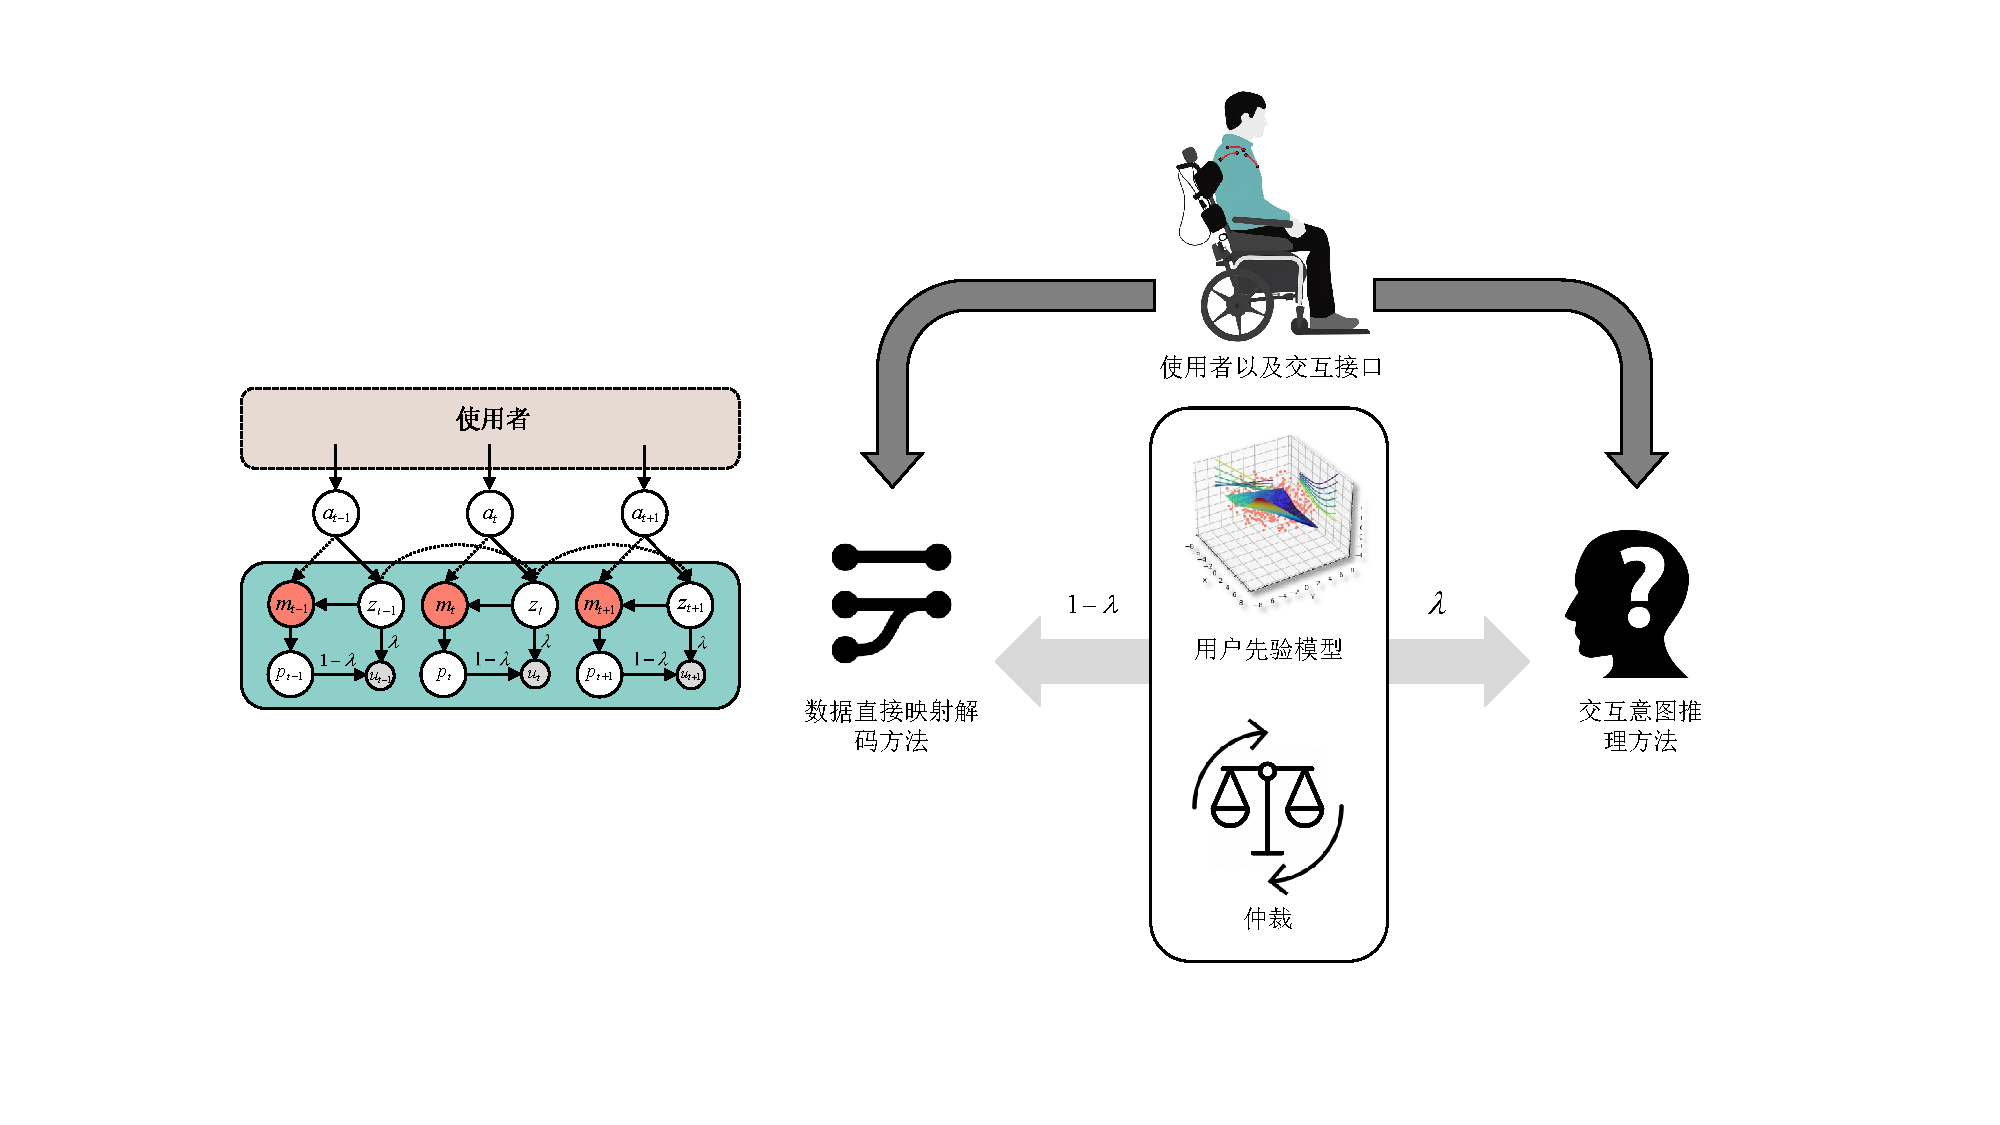
\includegraphics[width=0.55\textwidth]{3-Fig-9.pdf}
    \caption{基于共享自主的自适应命令映射解码方法的概率图模型}
    \label{3-fig-9}
\end{figure} 

\subsubsection{仲裁函数定义} 
通过将共享自主系统引入交互界面的解码过程,我们认为以基于确定性规则的数据解码方式为主的命令生成方式,辅以意图推理的自适应介入辅助可以实现操作指令在高动态性能表现下的同时提高其指令的准确性。为了实现解码方式的自适应切换,在该工作中通过将个性化先验知识嵌入到一个仲裁函数中来实现推理的自适应介入。图\ref{3-fig-9}给出了基于共享自主的自适应命令映射解码的概率图模型,其中用户的动作可以由基于确定性规则的数据解码(虚线)和基于不确定性意图推理的数据解码同时处理,并通过一个非线性仲裁函数实现自适应切换。特别地,由于所设计体-机交互界面在每个时刻都观察到${m_t}$,因此我们可以认为存在条件独立关系${z_t} \bot {p_t}|{m_t}$。共享数据解码方法输出的命令$u_t^{SCM}$定义为:

\begin{equation}
    \label{ex6}
    u_t^{SCM}\triangleq \lambda_t u_t^{UII}+(1-\lambda_t)u_t^{DCM}
\end{equation}   

其中$\lambda  \in [0,1]$是用于仲裁从两种数据映射解码方式的混合因子,共享自主系统的混合因子由预训练用户能力模型$\mathcal{F}(x)$动态调整。为了保证解码方式切换的平滑性,我们将其定义为一系列局部线性模型的加权线性组合,该方法也被称为感受野加权回归模型\cite{schaalScalableTechniquesNonparametric2002},定义如下式:

\begin{equation}
    \label{ex7}
    \mathcal{F} (x) \triangleq \frac{{\sum\nolimits_{k = 1}^K {{w_k}{g_k}(\hat x)} }}{{\sum\nolimits_{k = 1}^K {{w_k}} }}{\text{,  }}{g_k}(\hat x) = {\theta}_k^T{\hat x}
\end{equation}   
公式中$\hat x = {[\begin{array}{*{20}{c}}{{x^T}}&1\end{array}]^T}$,其中${x} \in {\mathbb{R}^2}$是二维命令空间中的位置向量,$K$是局部模型的数量,${g_k}(x)$是由${\boldsymbol{\theta }}_k^T \in {\mathbb{R}^{3}}$参数化的一阶线性多项式。权重${w_k\in {\mathbb{R}}}$根据一个径向基核函数计算:
\begin{equation}
    \label{ex8}
    {w_k} = \exp \left( { - 0.5 \times {{(x - {{c}_k})}^T}{{r}}(x - {c_k})} \right)
\end{equation}
其中$c_k$是径向基核函数的中心位置,参数$r$用于调整每个线性局部模型的感受野。每个局部模型的${\theta }_k$的参数可以通过实验中获得训练数据进行递归最小二乘得到。由于用户的表现会随着使用时间的增加而改变或提高,因此基于递归的优化允许通过增量学习的方式来更新模型。时间$t$处的混合因子的值定义为一个分段函数:

\begin{equation}
    \label{ex9}
    {\lambda _t} = \left \{{\begin{array}{*{20}{c}}
        {\begin{array}{*{20}{c}}
        0  \\  
        {\mathcal{F} (x)}  \\  
        1 
      \end{array}}&{\begin{array}{*{20}{c}}
        {,\mathcal{F} (x) < 0}  \\  
        {,0 < \mathcal{F} (x) < 1}  \\  
        {,\mathcal{F} (x) > 1} 
      \end{array}} 
      \end{array}} \right.
\end{equation}     

\subsubsection{用户能力模型建立}建立用户能力模型先验模型$\mathcal{F}(x)$的目的是希望明确使用者在命令空间中不同区域使用确定性映射规则进行指令生成的能力,但我们只能通过有限数量的实验来测试用户在不同空间位置的操控性能,因此可以通过一个目标跟踪任务中手机的用户的操作表现数据进行训练生成。由于本任务重所设计的命令空间为一个连续的二维平面,若要通过实验得到用户能力的量化表征,首先需要对命令空间进行离散化。  

根据菲茨定律\cite{tangFittsLawModulated2018},将光标移动到目标中心所需的时间受目标的大小以及光标与目标之间的距离的影响。通过保持目标的大小以及传输时间和相邻目标之间的距离恒定。我们通过受试者控制的光标与高亮标记的区域中心之间的欧氏距离度量来定义受试者使用基于确定性规则映射的数据解码方式的能力。如图XXX所示,该区域目标跟踪任务涉及记录在命令空间中的一个 0.8 厘米的受控光标和屏幕上一个$1\times1$cm大小的绿色高亮方形目标之间的距离值。目标在$20\times20$cm任务空间内(对应一个$5\times5$命令空间)以1秒的时间间隔以蛇形模式移动,参与者尽可能地使用肩部控制光标准确地跟踪高亮区域并保持光标在目标的指定区域内,在显示器上通过显示一个受控的蓝点光标提供实时视觉反馈,其中光标的位置$s$与目标$g$中心之间的欧几里德距离是在高亮方形目标开始转移到下一个位置时计算的,因此在一轮实验中将产生400个数据点。

\begin{equation}
    \label{ex12}
    d \triangleq \frac{1}{1+e^{-8\sqrt{(g-s)^T(g-s)}+4}} 
\end{equation}    
此处,$d$为一个非线性Logistic函数,其将偏移欧式距离度量的结果限制在0到1的范围内来量化用户的表现。在实验中,我们要求每名参与者完成三次任务,最终我们将得到每次实验命令空间中与目标位置   $g_c$相关的1200组数据$[g_c,d]$。先验模型$\mathcal{F}(x)$由25个线性模型$g_k(\hat x)$组成,其中每个线性局部模型的中心$c_k$以2的间隔均匀分布在命令空间中。

\section{实验流程与设置}基于所设计交互界面和数据解码方法,我们通过一系列操作任务来评估不同解码方法的表现。5名健康受试者(年龄:$26\pm3$;性别:3男2女;身高:$174\pm16$cm;体重:$67\pm17$kg)参与了本研究并签署知情同意书。所有参与者在实验前都对所设计交互设备进行了为期3天的了解使用,以熟悉操作方法。我们要求所有受试者将他们的小臂和手放在桌子上保持固定,以模拟上肢残疾的患者。

\subsection{实验任务}   
    \subsubsection{八方向目标到达任务}在本任务中,参与者需控制直径为0.8厘米的蓝色光标,并将其移动至八个预定义的固定目标。每个目标的直径为2.4厘米,且以45度为间隔,位于直径26厘米的圆上。当用户将光标移至位于命令空间中心的中心目标时任务将启动。任务目标从最右边的区域开始,按照逆时针顺序依次激活目标。为完成每个任务环节,用户需将光标保持在目标内至少2秒。若用户在12秒内未完成一个环节,目标将自动切换至下一个,且该任务环节将被视为失败。

   \subsubsection{随机目标到达任务}在本任务中,通过在直径为26厘米的圆上均匀分布的采样,我们随机生成了8个目标。任务过程类似于``八方向目标到达任务'',用户需将光标导航至随机生成的目标区域,之后将其返回到根目标。

   \subsubsection{虚拟动力轮椅驾驶任务}电动轮椅作为一种移动辅助设备,是残疾人辅助器具中最为重要的一种。本研究基于两轮差速移动机器人模型,构建了虚拟动力轮椅驾驶场景。图XXX展示了所开发的虚拟场景。在该任务中,参与者需要在尽可能短的时间内驾驶虚拟轮椅穿越一系列障碍。  

\subsection{不同传感器配置模式的消融对比实验} 多模态方法在提升物体信息获取准确性方面已受到广泛的认可和应用,例如医疗决策辅助系统和组合导航系统\cite{williamsonContinuousUncertainInteraction2006}。此类方法可通过利用额外的模态数据为推断算法积累可以用于推断意图的证据。然而,目前尚未明确冗余的感知信息能否显著提升人机交互接口的性能。为了探究这一问题,在我们在研究中设计了一项消融实验,旨在探讨各种传感器配置对意图推断过程的影响。表\ref{tab3-1}列出了六种预设的传感器配置。我们要求所有参与者针对每个传感器配置完成``八方向目标到达任务''五次,并在传感器配置发生改变时重新训练交互意图推理解码模块。为了减轻疲劳对实验结果的影响,我们在每项任务之间给参与者提供了2分钟的休息时间。 

\begin{table}
    \centering
    \caption{用于意图推理的传感器数据源配置模式}
    \setlength{\tabcolsep}{3pt}
    \begin{tabular}{c p{180pt} c }
    \hline\hline
    配置模式代号 & 数据源使用 & $N$ \\ 
    \hline
    OS& 仅拉伸数据& 4 \\ 
    BS& 拉伸和弯曲数据&12 \\ 
    GS& 陀螺仪+拉伸数据&7 \\ 
    GBS& 陀螺仪+拉伸和弯曲数据&15 \\ 
    AGS& 加速度计+陀螺仪+拉伸数据&10 \\ 
    AGBS& 加速度计+陀螺仪+拉伸和弯曲数据&18 \\ 
    \hline\hline
    \end{tabular}
    \label{tab3-1}
\end{table}     

\subsection{不同数据解码方法的比较} 每位参与者按顺序完成了八方向目标到达任务、虚拟动力轮椅驾驶任务和随机中心向外目标到达任务,每项任务均进行了五次。为确保任务结果的公正性,参与者未获知解码方法的具体技术细节,仅知道所使用方法的名称。为适应新的解码方法,我们给予参与者2分钟的时间来熟悉在任务空间中的操作。此外,在进行电动轮椅驾驶任务之前,我们确保每位参与者通过使用设计的交互接口和标准的轮椅操纵杆来熟悉驾驶任务。参与者按以下顺序使用两种交互接口完成任务:操纵杆、基于确定性规则映射的命令解码、基于不确定性意图推理的命令解码以及共享自主切换的数据解码方法的柔性交互接口。每个参与者执行任务三次。 

\section{实验结果与分析}     

\subsection{交互效果评价量化指标}   
 \subsubsection{完成任务花费的时间(TS)}该指标涉及用户从任务空间中心移动光标至目标位置所需的持续时间。较短的移动时间反映了解码算法的准确性和效率的提高。
 \subsubsection{平均轨迹偏移距离 (AveOD)}该指标评估了光标相对于连接中心目标和激活目标之间直线路径的平均偏移量,用于反映光标在任务空间中移动的线性程度。较高的``AveOD''值表明光标经常偏离用户期望的路径,从而需要用户投入更多的精力来控制光标。
 \subsubsection{平均光标移动速度(AveSpeed)}该指标是根据用户控制光标的平均速度计算得出的。 “AveSpeed”值越高表示接口具有越高的动态性能。
 \subsubsection{平均光标运动急动度 (AveJerk) }该指标是通过计算用户在任务空间中控制的光标位置相对于时间的三阶导数来确定的。较高的``AveJerk''值表明用户对光标的控制不够平滑,并且存在较多抖动。在这种情况下,``抖动''指的是光标发生的不可预测的小而快速的移动。  

\subsection{最优传感器配置模式}图\ref{fig:3-10}(A)为使用柔性体-机交互接口的参与者在不同传感器配置下执行实验任务的表现量化指标的分布情况。图\ref{fig:3-10}(B)显示了被控制光标在任务空间中一些典型的运动轨迹。在数据分析中我们使用了单因素方差分析方法进行统计显著性分析。实验数据表明,与OS配置模式相比,使用BS传感器配置方法的操控表现提高并不显着。尽管将柔性传感器的弯曲数据用于交互意图推理并相较于OS模式在一定程度上改善了动态性能(平均``AveSpeed''从0.141m/s增加到0.149m/s),但也导致了操控线性度的下降(平均``MaxOD''从2.06cm上升至2.28cm)。这一发现表明,使用柔性传感器的弯曲信息可能会在交互意图的推理中中引入更多的不确定性因素,这是因为某些软传感器在肩部运动期间可能会使得交互接口在无意中向不可预测的方向弯曲导致的。在GS模式中,陀螺仪数据的加入显着提高了任务的完成效率($p<0.001$)。与仅使用柔性传感器拉伸信息的OS模式相比,GS模式具有较低的``TS''表现(平均2.11秒)和较高的``AveSpeed''表现(平均0.16 m/s)。此外,使用GS配置模式还降低了``TS''和``MaxOD''指标的的标准差,并且光标移动的轨迹表现出相较于其他模式更好的线性度。这主要归功于陀螺仪的具有较高的动态性能表现,此外陀螺仪仅检测使用者上半身的整体相对运动,而不是肌肉活动,因此减少了穿戴式交互接口中不确定性因素的影响。使用了三种传感器信息的GBS配置模式并没有显着提高意图推理控制光标的性能。相反,与之前分析的原因类似,虽然与``GS''模式相比,它在一定程度上提高了``AveSpeed''的表现($p<0.01$)。但是其仍然会导致任务完成效率和平滑度表现变差,体现在GBS模式拥有较高的``TS''($p<0.001$)和``AveJerk''($p<0.001$)值。

\begin{figure}[!t]
    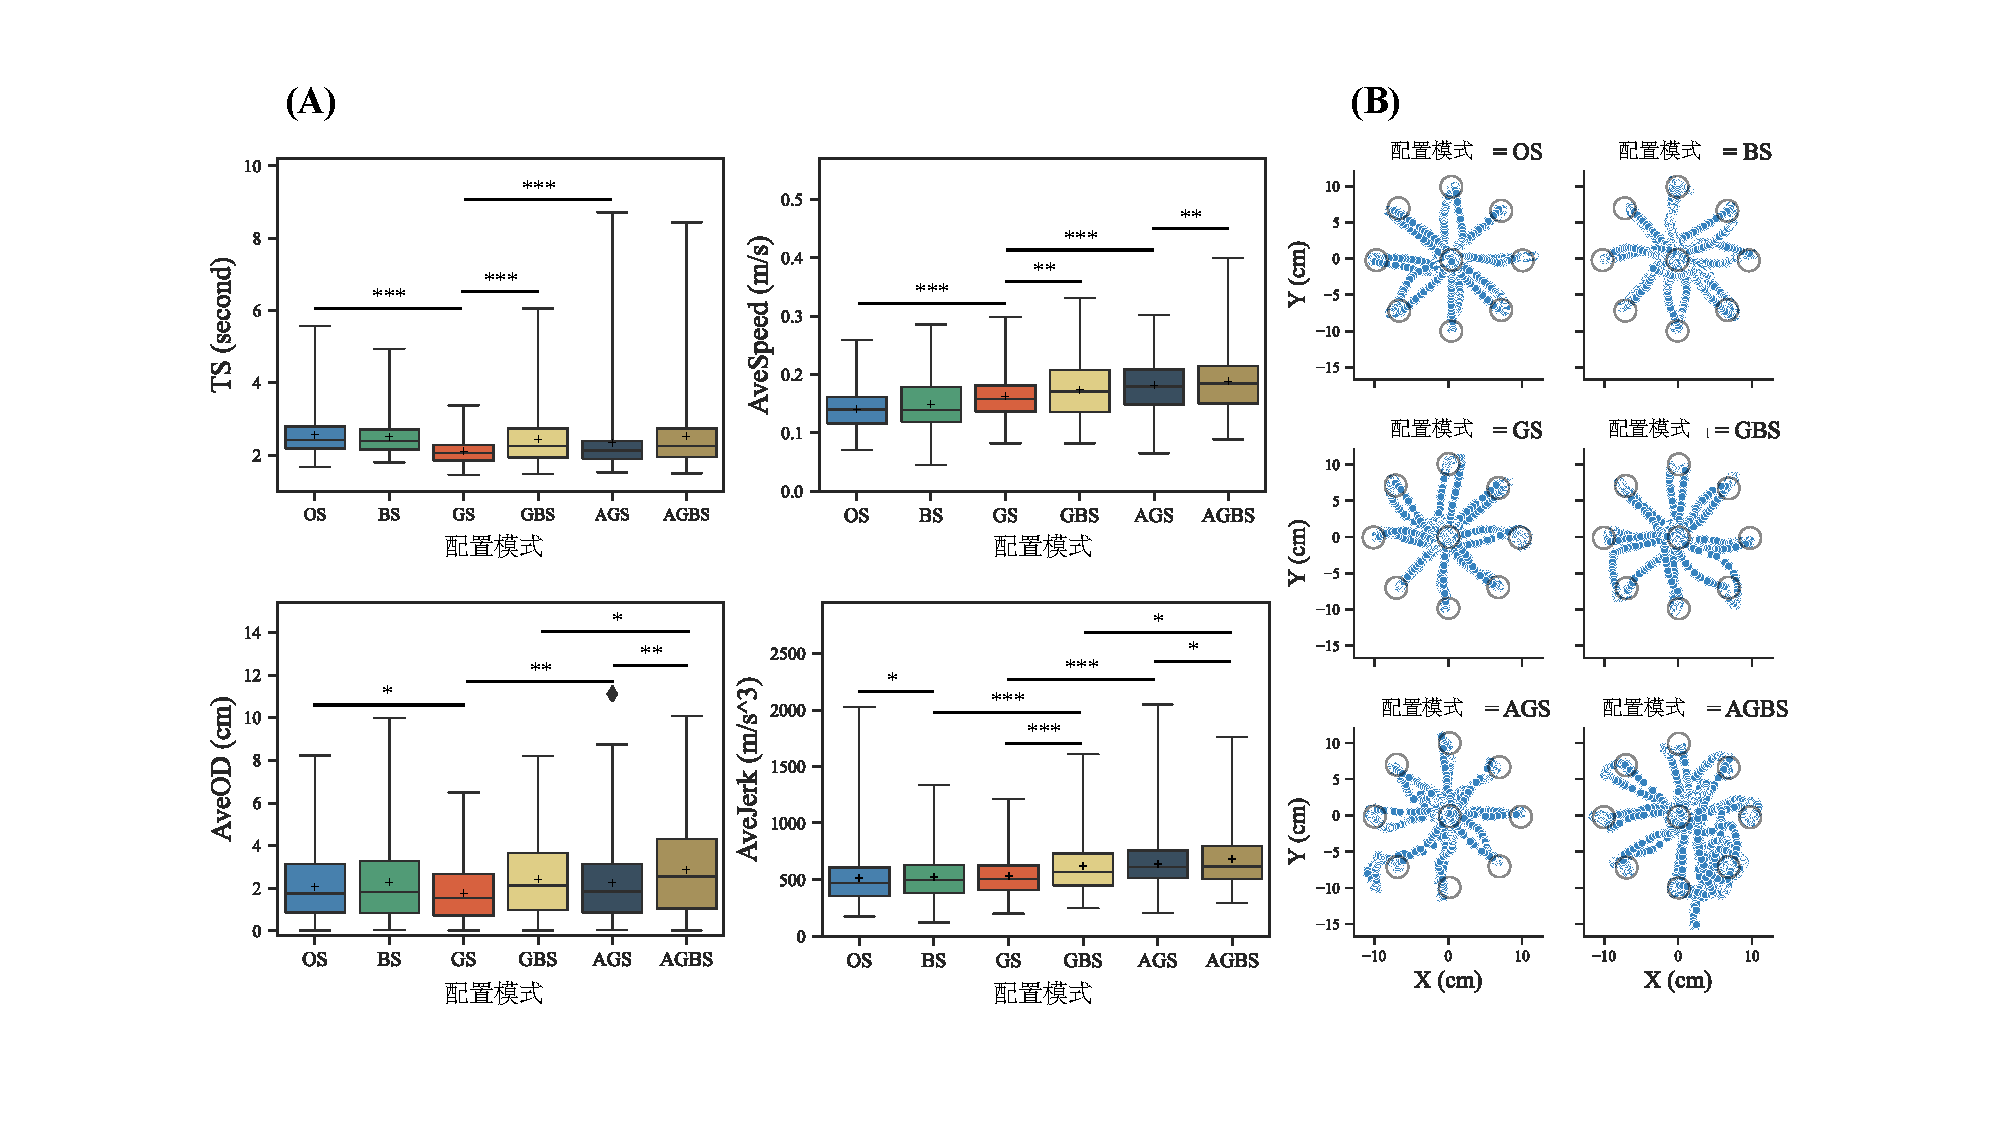
\includegraphics[width=1\textwidth]{figures/3-Fig-10.pdf}
    \caption{(A) 最佳传感器配置实验中不同配置的性能, 其中``*''代表$p<0.05$,``**''代表$p<0.01$,``***''代表$p<0.001$。 (B) 不同传感器配置下``8 方向中心向外目标到达任务''的任务空间轨迹。}
    \label{fig:3-10}
\end{figure}  
加速度计的使用可最大化所有配置中``AveSpeed''的值(其中AGS配置模式为 0.181 m/s,AGBS模式为0.188 m/s),但是其同样也会增加时间花费``TS''的方差。与没有使用加速度计进行意图推理的GS和GBS配置模式相比,AGS和 AGBS模式的线性度和平滑度相对较差,体现在他们具有明显更高的``MaxOD''($p<0.01$)和``AveJerk''($p<0.05$)。如图\ref{fig:3-10}(B)所示,我们发现AGS和AGBS的光标轨迹明显比其他配置模式更加混乱,这是因为实验参与者在操控任务空间中的某些区域无法很好地控制光标,导致需要频繁修正光标的位置所导致的。此外,我们发现在使用意图推理进行光标操控时,当不使用加速度计时所有参与者都在指定的时间内成功完成了目标到达任务。然而,我们观察到一些参与者在实验中无法使用AGS和AGBS配置完成任务。之所以会出现这个问题,是因为加速度计作为一种绝对量传感器,对用户的上半身的绝对姿态较为敏感。因为我们假设用户的意图与交互接口的传感器测量之间存在线性关系,即使使用者身体姿势的微小调整也会对意图推断产生重大影响。它会导致生成的命令经常偏离用户的意图,使参与者难以保持对光标的控制。  

综合来看,消融实验的结果表明仅使用陀螺仪角速度信息和柔性传感器拉伸信息的GS配置模式表现出最综合的性能优势,其具有更为优异的任务完成效率和线性度,同时保持适度了对光标操控的动态性能。因此,我们选择GS模式作为实验的基准配置。
\begin{figure}[!t]
    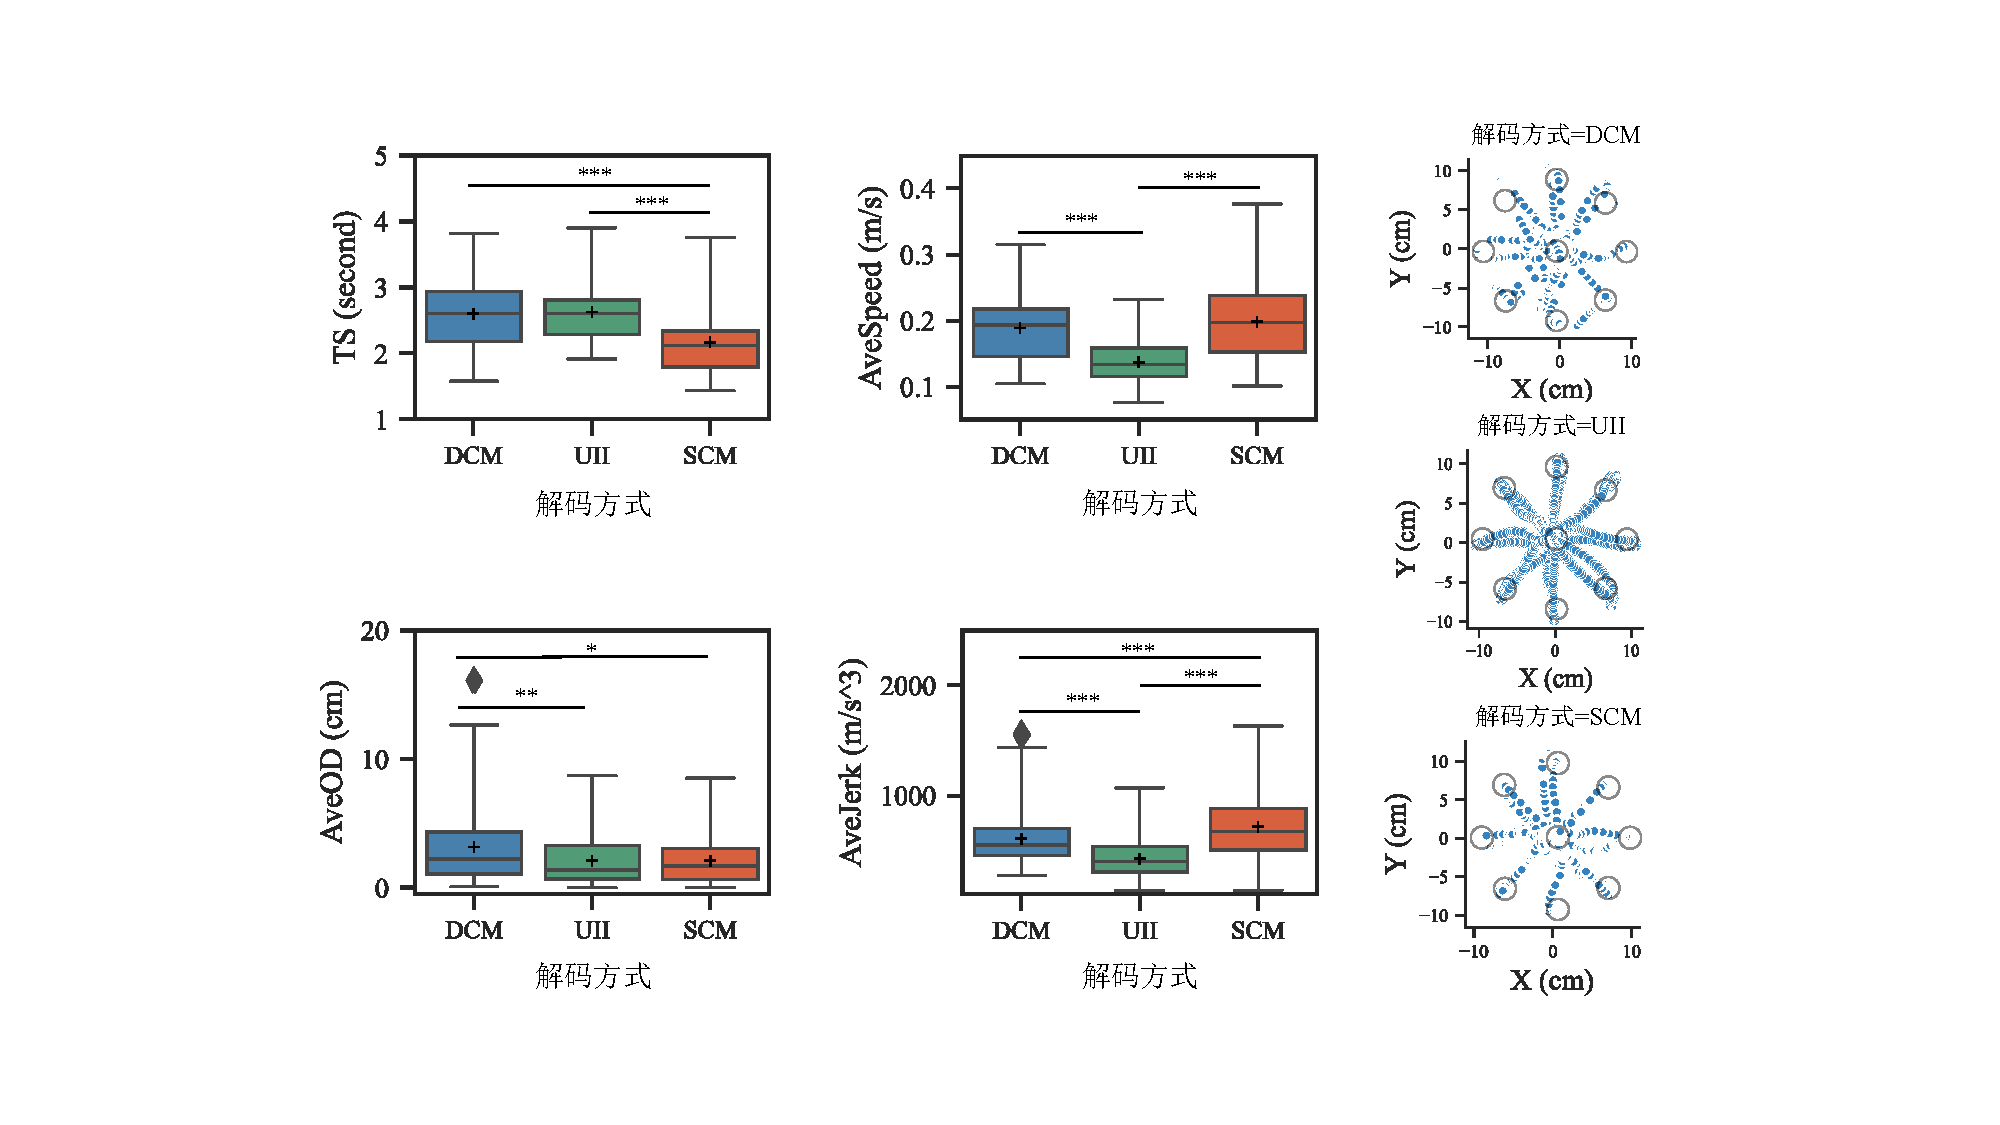
\includegraphics[width=1\textwidth]{figures/3-Fig-11.pdf}
    \caption{五名受试者的在感受野参数$r$由0.5导2.5设置下的用户能力模型热图}
    \label{fig:3-11}
\end{figure}  
\subsection{基于用户能力模型的仲裁函数}共享自主系统用于切换解码方式的仲裁函数是基于一个由操控实验数据建模的非线性模型的。模型的感受野大小影响了指令解码切换的平滑度。图\ref{fig:3-11}给出了当感受野$r$从0.5增加到2.5时,五名参与者的能力模型的变化。通过选择合适的局部模型参数,我们可以实现泛化的$\mathcal{F}(x)$,从而在解码方式的切换过程中防止权重$\lambda_t$的突然变化导致的光标抖动。当$r=0.5$时,由于感受野过小因此无法建立可用的$\mathcal{F}(x)$,使其不适合用于共享自主的在线仲裁切换。随着感受野$r$半径的增加,模型泛化性能不断的提高,然而,过大的感受野可能会导致模型表现出过度平滑效果,导致其丢失局部特征。因此,在应用中需要平衡模型泛化性和保留局部特征这一,作为基准在本章中统一设置参数$r=2.2$。此外,我们观察到不同参与者的$\mathcal{F}(x)$表现出一些共同的特征。从图\ref{fig:3-11}中可以看出,五名实验参与者在命令空间中的第一象限通常表现最出色,但在第四象限表现最差。这可能是由于柔性体-机交互设备的设计缺陷所导致的,位于右肩的软传感器比左肩涉及更多的不确定性干扰,参与者在控制光标时遇到挑战。另外,我们观察到,与第一和第二象限相比,参与者在第三和第四象限的表现较差。这一观察结果与肩部运动的直观本质相一致,参与者表示控制肩部向前移动通常比向后移动更容易进行对光标的精确控制。  

\subsection{不同解码方法的实验表现}     

\begin{figure}[!t]
 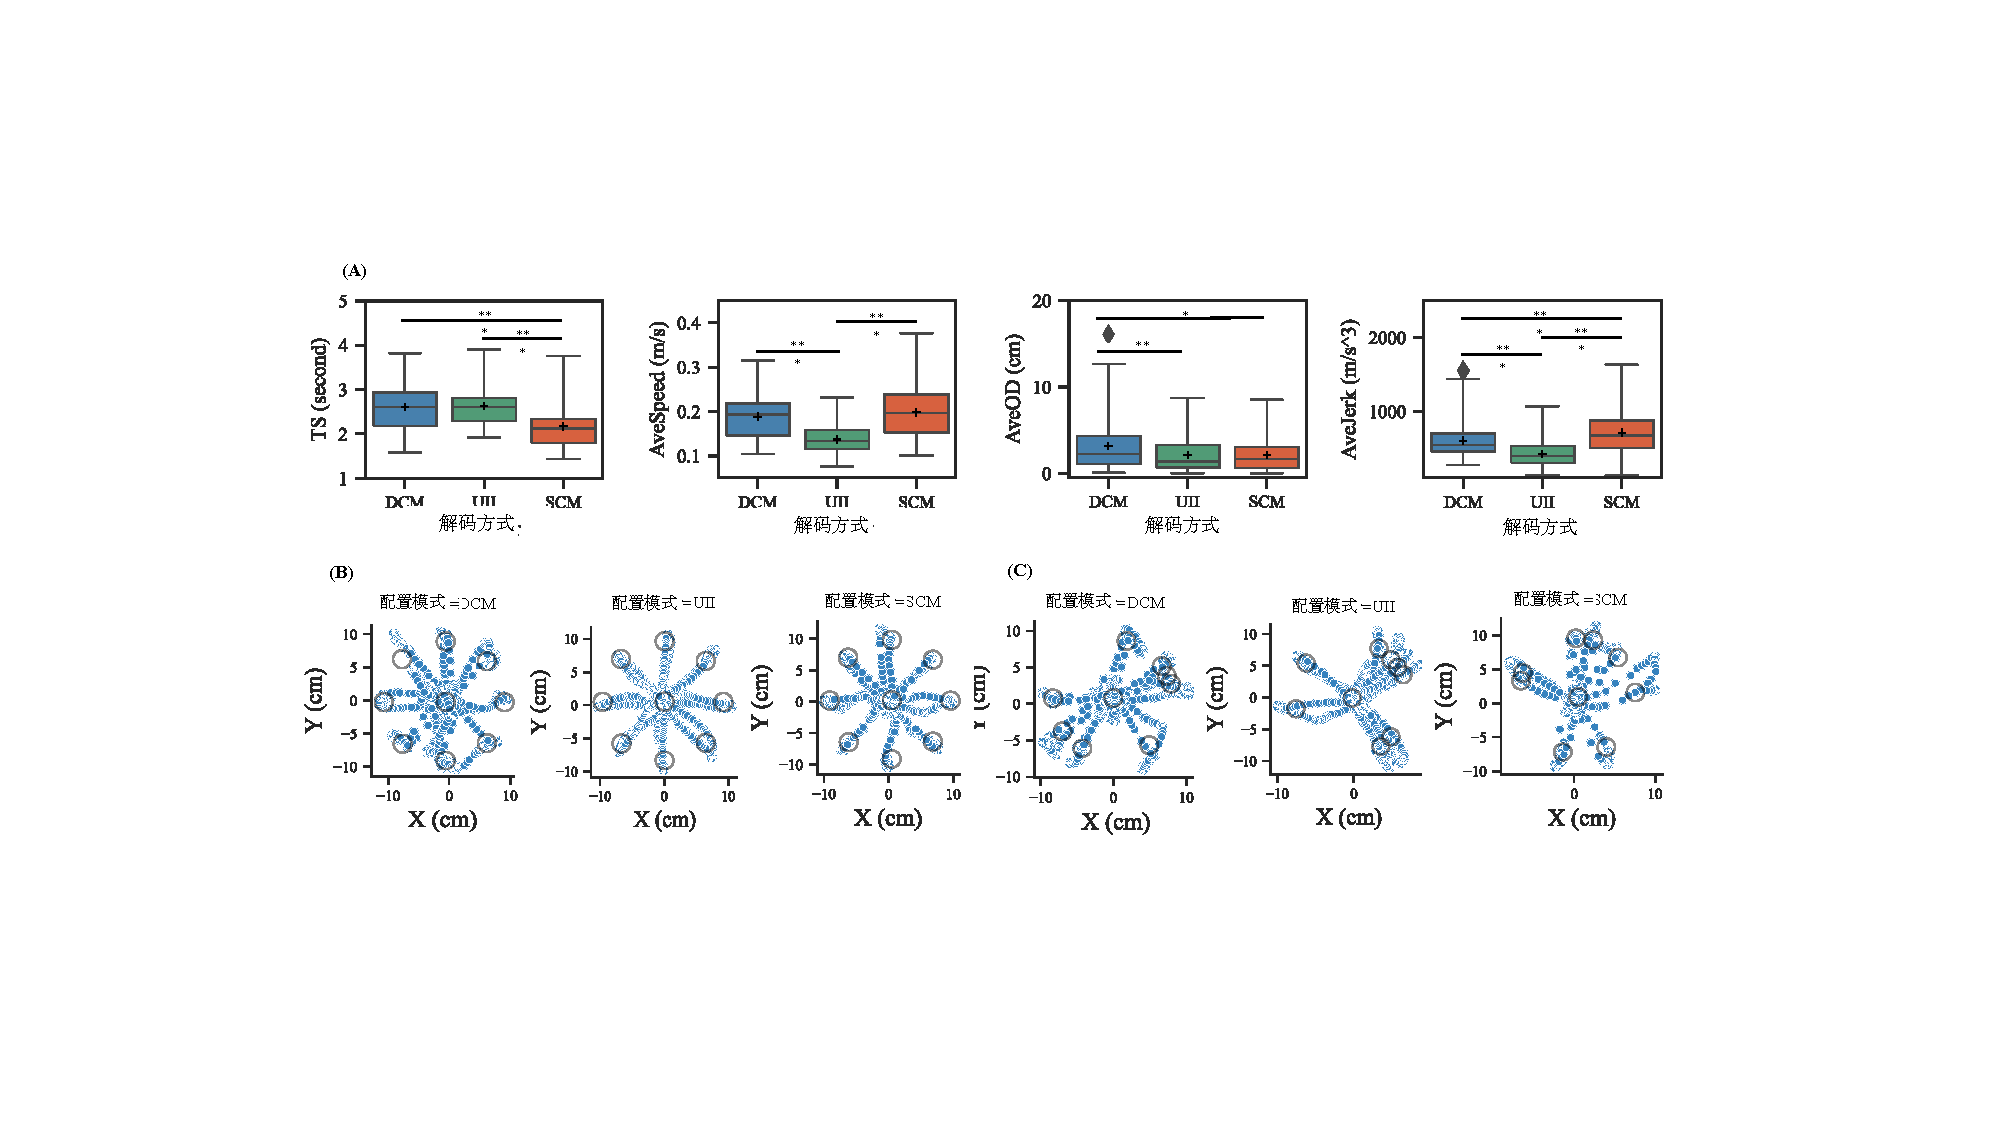
\includegraphics[width=1\textwidth]{figures/3-Fig-12.pdf}
 \caption{(A) 不同解码方法在“8 方向中心向外目标到达任务”中的性能。 (B)“8方向中心向外目标到达任务”中不同解码方法的轨迹。 其中“*”代表$p<0.05$,“**”代表$p<0.01$,“***”代表$p<0.001$。  }
 \label{fig:3-12}
\end{figure}     

\begin{figure}[!t]
    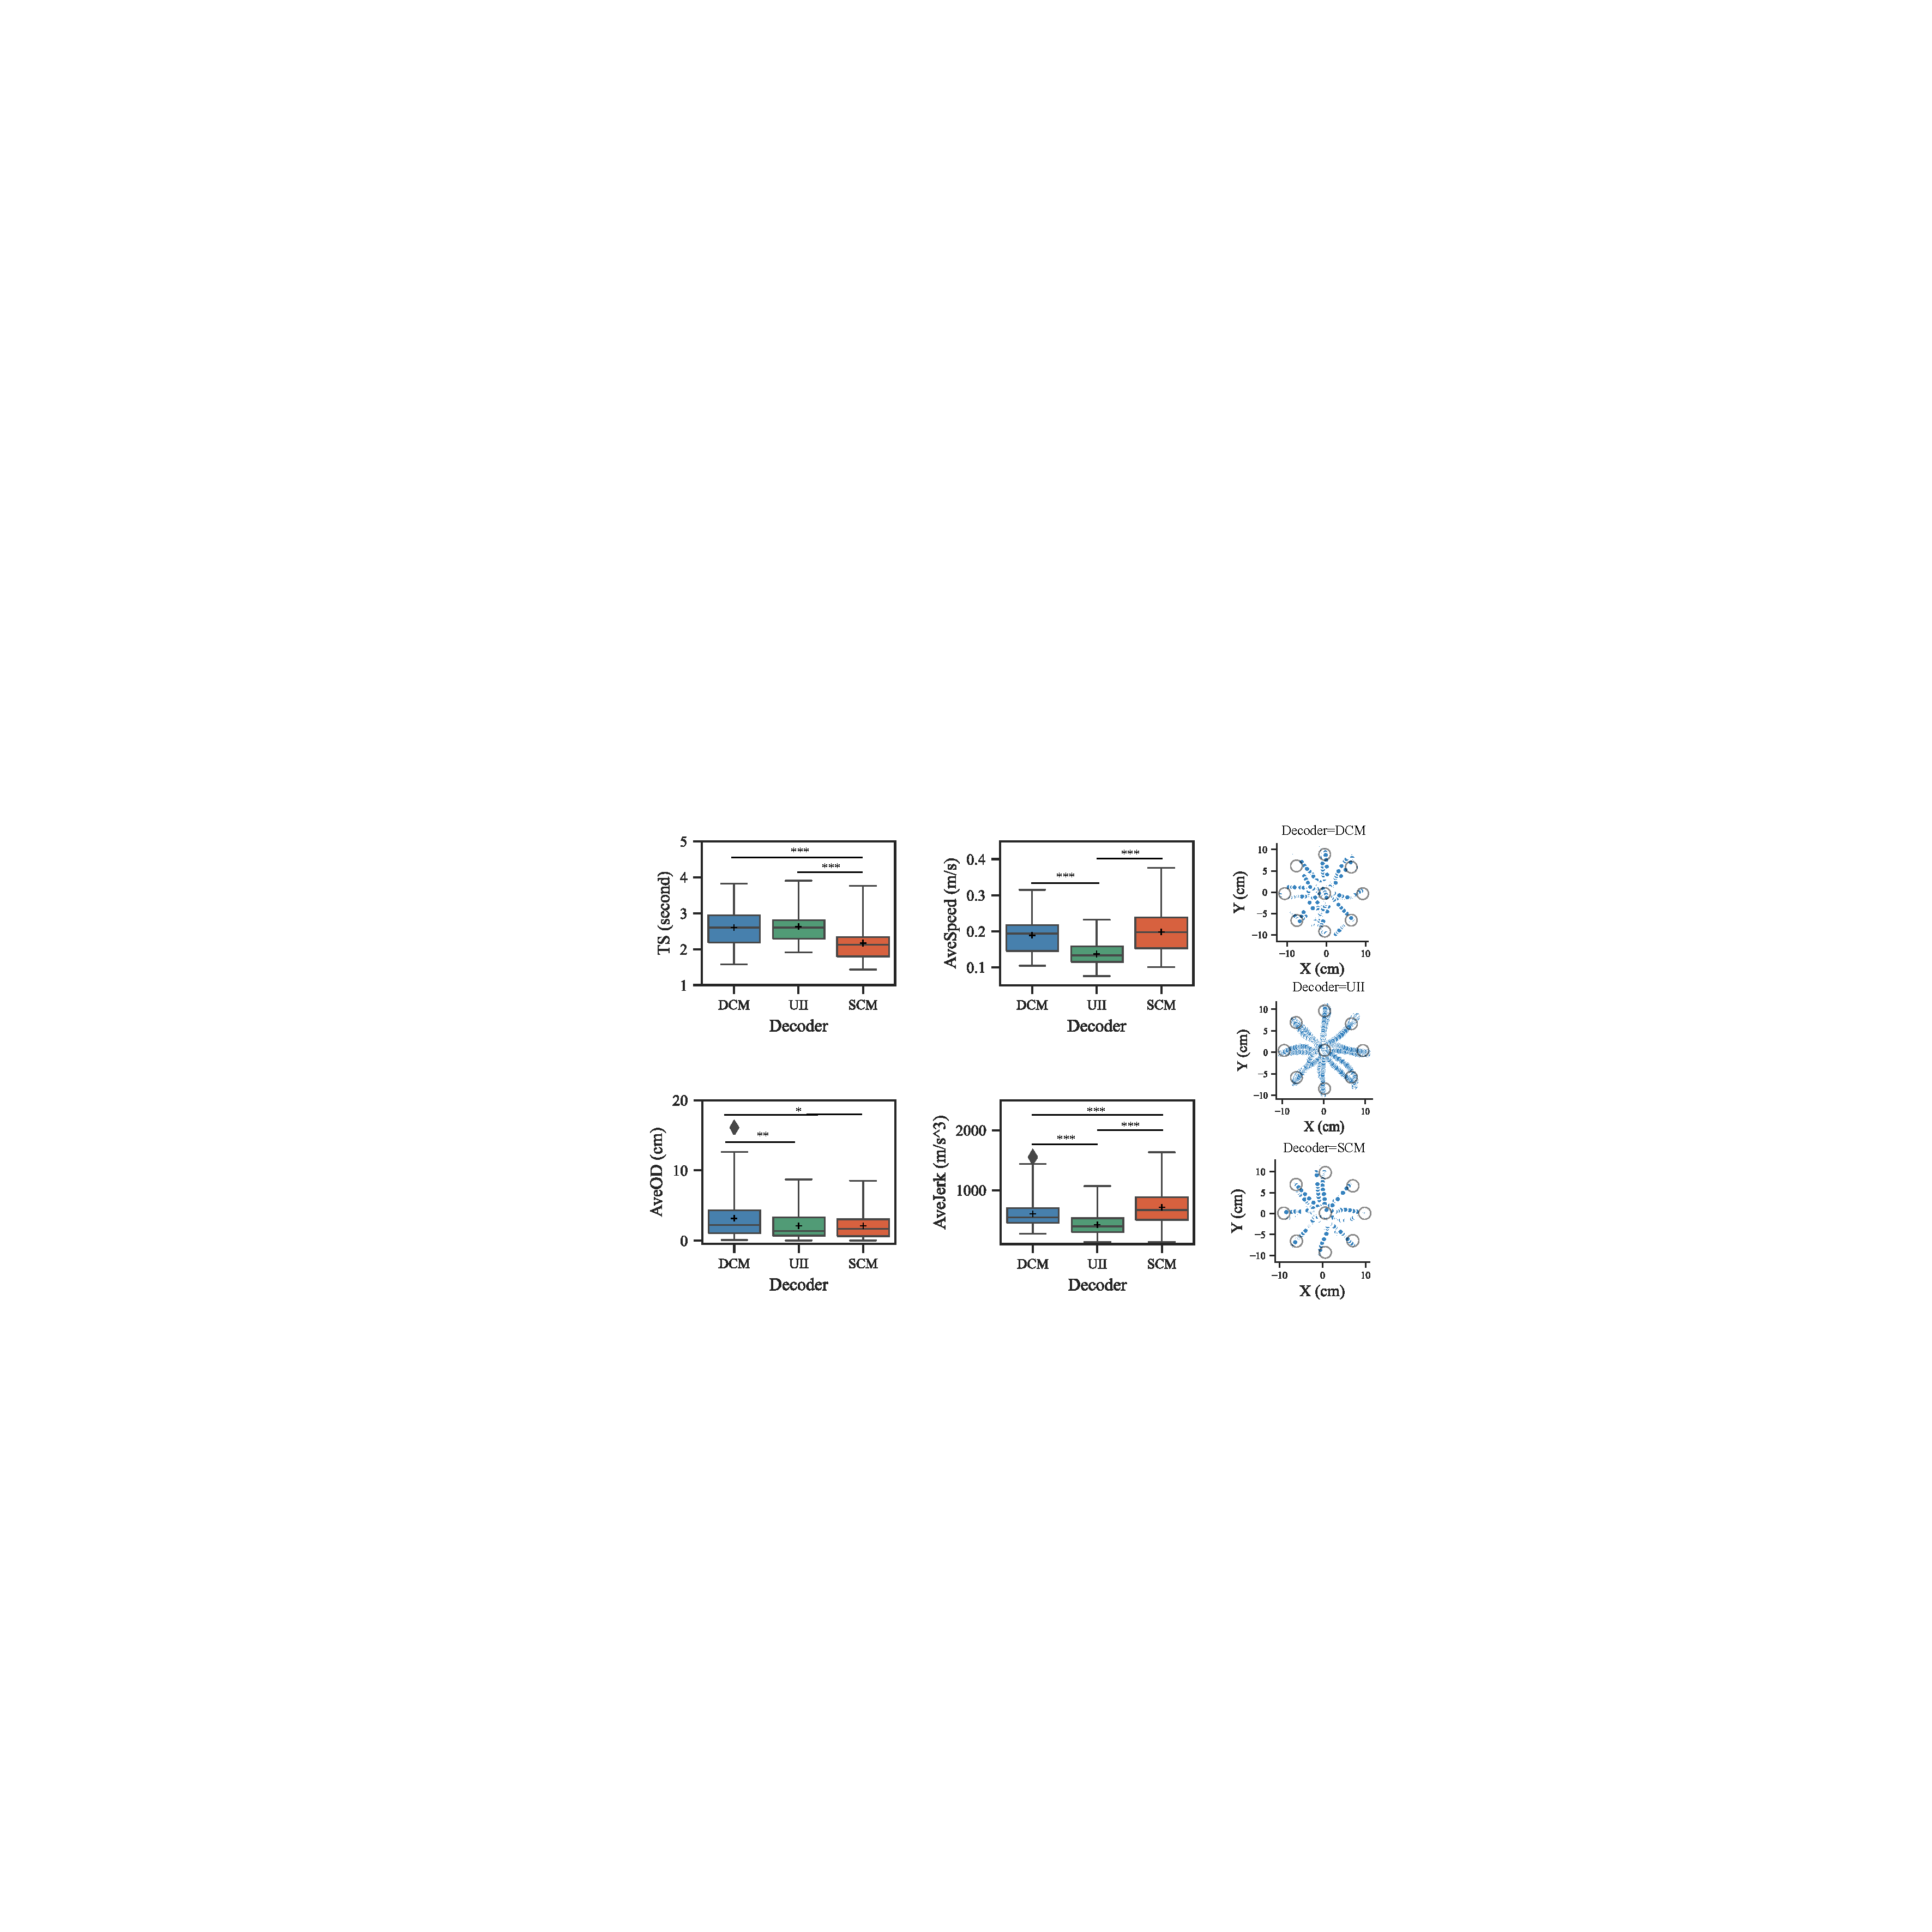
\includegraphics[width=1\textwidth]{figures/3-Fig-13.pdf}
    \caption{(A)“随机中心向外目标到达任务”中不同解码方法的轨迹。 (B) “随机中心向外目标达成任务”的象限 I/II 和 III/IV 中的表现。 其中“*”代表$p<0.05$,“**”代表$p<0.01$,“***”代表$p<0.001$。  }
    \label{fig:3-13}
\end{figure}  

\subsubsection{八方向目标到达任务实验表现}图\ref{fig:3-12}(A)显示了前文中所提到的三种不同数据解码方法在八方向目标到达任务中的实验表现。相较于其他两种解码方式,尽管基于确定性规则直接映射解码模式(DCM)在``AveSpeed''($p<0.001$)指标方面具有优势,但与意图推理模式(UII)相比并没有显着改变任务完成时间花费指标``TS''。这是因为使用直接映射解码的参与者经常超越任务目标的中心位置(如图\ref{fig:3-12}(B)所示),因此参与者往往需要更多的时间来调整操控光标,使其保持在激活的环形目标的范围之内导致降低了任务完成效率。此外,在实验中我们发现由于柔性传感器的在使用者运动中的不确定性形变常常会导致光标向使用者意想不到的方向移动。然而,交互设备使用者通常能够借助显示屏的视觉反馈快速调整光标的位置,但这会在一定程度上增加他们的认知负担。  

意图推理需要更多的来自传感器的证据积累,这导致其与直接的数据映射动态性能的下降。尽管存在这一缺点,意图推理方法(UII)在光标移动线性度``AveOD''($p<0.01$)和平滑度``AveJerk''($p<0.001$)方面表现出了显着的优势。与DCM模式相比,从其较低的``AveOD''和``AveJerk''值可以明显看出这一点。 基于不确定性意图推理的方法的光标操控运动轨迹通常更直接地到达目标,需要参与者较少的实时纠正和调整。这表明意图推理方法在控制光标方面提供了更好的准确性和精度。与基于规则的直接数据映射方式相比,意图推理虽然显着降低了``AveSpeed''的值,但提高了任务完成的效率,这从两种方法之间相似的“TS”性能中可以明显看出(在更低的平均速度下,拥有相似的任务完成效率)。意图推理的这一特性通过最大限度地减少光标操作过程中对于控制结果反馈校正或微调的需要,增强了整体用户体验。  

基于共享自主的自适应解码方案(SCM)与DCM模式具有类似的``AveSpeed''性能表现,但是显着降低了实验中的``TS''值($p<0.001$),这表明使用SCM模式相较于DCM模式具有更好的任务完成效率。此外,SCM模式和UII模式在光标操控线性度指标``AveOD''上具有相似的性能,但是其明显优于DCM模式($p<0.05$)。这表明,SCM在一定程度上结合了DCM的高动态特性和UII的高精度特性。在实验任务中,实验参与者表示在使用自适应解码方案时时可以清晰地感受到意图推理辅助的干预。在用户使用DCM模式表现良好的区域,SCM使得用户主要使用DCM来控制光标因此保证了操控的高动态性能。反之,在参与者使用DCM模式表现不佳的区域,共享自主解码方式将操控模式无缝切换至意图推理,通过降低一定的动态性能进而保证光标控制的准确性。然而,在自适应切换过程中也带来了一个问题,即被控制的光标由于仲裁函数的对于解码方式的动态调整而容易产生一些抖动。因为与DCM和UII模式相比,SCM模式具有明显更高的``AveJerk''值($p<0.001$)。  

\subsubsection{随机目标到达任务实验表现}在具有固定目标位置的八方向目标到达任务的基础上我们进一步测试了使用者使用三种解码方法在任务空间不同区域到达随机目标的表现情况。图\ref{fig:3-12}(C)显示了一位参与者的任务空间中的一些代表性光标轨迹。与具有更高``AveSpeed''值的UII模式相比,参与者使用DCM模式通常需要更多时间($p<0.01$)来完成任务。SCM显示出明显低于 DCM 和 UII 的任务花费``TS'',表明其相较于其他两种解码模式显著提升了任务的完成效率($p<0.001$)。 基于意图推理的方法仍然具有最好的线性度和平滑度,表现在其仍然具有最低的``AveOD''和``AveJerk''值。如图\ref{fig:3-13}(A)和(B)所示,我们进一步分析了参与者使用SCM解码方式控制光标分别达到位于象限I/II和象限III/IV的目标的表现。在任务空间的象限I/II 中,SCM与DCM模式具有相似的性能。在象限 III/IV 中,尽管会引起一些抖动,SCM模式相较于UII模式在明显提高了平均速度``AveSpeed''的基础上($p<0.05$),同时保持与UII类似的操控线性度指标``AveOD''。综合来看,SCM模式通过将预实验中用户使用DCM模式的表现先验知识纳入到一个共享自主自适应框架中,实现了由动态性能较高的直接数据映射到更加准确平滑的意图推断解码的无缝切换,在保证了操控动态性能的前提下确保了生成命令的准确性。  

\subsubsection{虚拟动力轮椅驾驶任务实验表现}     
  
\begin{figure}[!t]
    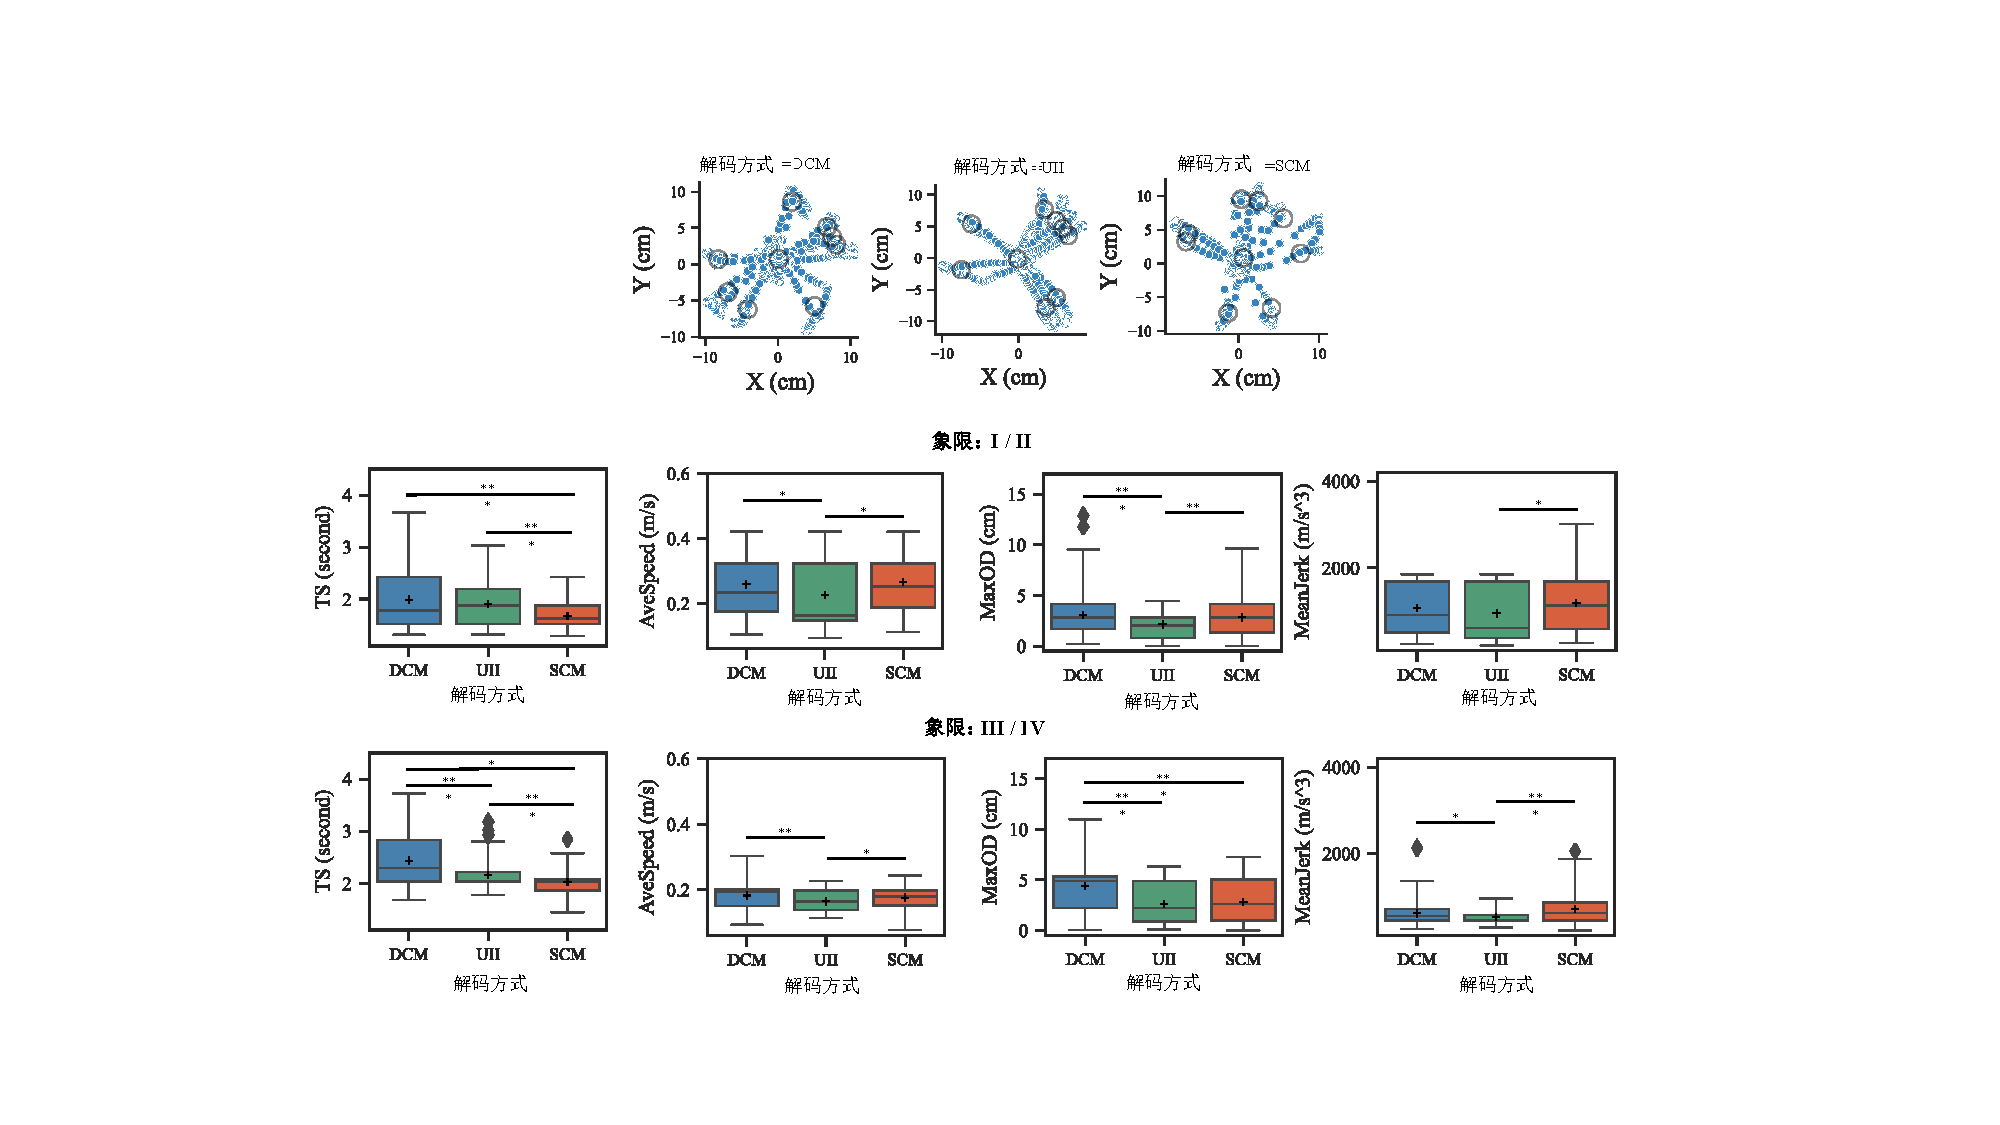
\includegraphics[width=1\textwidth]{figures/3-Fig-14.pdf}
    \caption{(A) 虚拟电动轮椅驾驶场景的 3D 渲染。 (B) 由 SoftBoMI 的操纵杆和不同解码器控制的虚拟电动轮椅的轨迹。红十字表示发生碰撞。 (C) 在轮椅驾驶任务的命令空间中生成命令。蓝色区域是死区。}
    \label{fig:3-14}
\end{figure}  

图\ref{fig:3-14}(B)描绘了轮椅在虚拟场景中的运动轨迹。表二提供了实验性能的概述。当使用操纵杆时,参与者的完成时间较短,平均为 30.93 秒,并且遇到的平均碰撞次数最少,约为 3.4 次。操纵杆突出的触觉反馈有助于平稳、精确地控制虚拟轮椅,使参与者能够沿直线操纵它并轻松进行微调。 DCM 的性能与操纵杆类似,但控制精度较低,因此更容易在狭窄空间内发生碰撞。  

\begin{table}
 \centering
 \caption{虚拟电动轮椅驾驶的性能  }
 \setlength{\tabcolsep}{5pt}
 \begin{tabular}{c c c}
 \hline\hline
  Interface & Average Time Spent & Average Number of Collisions  \\  
 \hline
 JoyStick&        $30.93\pm 2.43$        s&        $3.4$         \\ 
 DCM&        $31.46\pm 2.26$        s&        $5.8$         \\ 
 UII&        $35.38\pm 1.63$        s&        $61.8$         \\ 
 SCM&        $31.12\pm 1.03$        s&        $11.6$         \\  
 \hline\hline
 \end{tabular}
 \label{tab3-2}
\end{table}     

参与者在使用 UII 时表现最差:他们完成任务的时间最长,并且经历了更多的碰撞。如图3(I)所示,在任务开始时的直线行驶过程中,UII的轮椅轨迹有明显更高的振幅振荡。这是因为UII显着增加了整个闭环控制系统的延迟。大多数参与者需要很长的调整时间才能稳定轮椅。由于高延迟,他们必须隐式地建立对肩部和 SoftBoMI 动态的内在信念,但在复杂的肩部运动中实现这一点可能具有挑战性。  

另外,我们观察到 SCM 和 DCM 的性能相似。与 UII 相比,这两种方法在闭环系统的动态性能方面都表现出了显着的优势。然而,SCM并没有显着提升整体性能。这是因为设计的虚拟场景不存在需要快速转向的区域。因此,单片机产生的命令主要集中在命令空间的第一象限和第二象限(如图6(C)所示)。正如上一小节所讨论的,SCM 在这些区域中更喜欢使用 DCM 进行解码。尽管如此,某些区域仲裁切换引起的抖动仍然会影响虚拟轮椅的控制精度。这从 SCM 比 DCM 发生更多冲突的事实可以明显看出。  

总而言之,人机系统中的控制不仅仅是用户将观察到的状态与预期状态进行比较的问题。它还取决于受控系统的未来响应。如果系统中的延迟像 DCM 和 SCM 一样短,则简单的比较器控制器将运行得相当好;这允许用户将系统的延迟时间隐式建模为常数。对于更长的延迟,用户将建立更复杂的预测模型。例如,我们发现参与者在使用 UII 时往往会从连续控制降级为发出短信号的突发控制。由于虚拟轮椅的预期状态和当前状态之间的一些小偏差,常常会导致用户失去对轮椅的稳定控制。为了避免碰撞,他们往往会降低行驶速度以保持稳定的控制。  

\subsection{用户研究}用户研究为 SoftBoMI 解码方法的性能提供了有价值的附加视角,并帮助我们进一步验证所提出方法的有效性。在完成目标到达任务和虚拟轮椅驾驶任务后,参与者被要求提供首选解码方法的名称。  

\subsubsection{在目标到达任务中参与者表示更喜欢基于共享自主切换的自适应解码方法}七名参与者表示相对于 DCM 和 UII 更喜欢 SCM,理由是其卓越的动态性能和准确性。使用 DCM 时,光标经常偏离到非预期位置,尤其是在命令空间的第三和第四象限中,而此问题在第一和第二象限中出现的频率较低。它导致 SoftBoMI 对于参与者来说变得“不可预测”。然而,当任务完成时间不是优先考虑的时候,参与者可能会选择 UII,因为它提供更流畅、更准确的命令生成。  

\subsubsection{在虚拟电动轮椅驾驶任务中,参与者更喜欢 DCM 和 SCM 而不是 UII  }    五位参与者表示偏好 DCM,四位参与者偏好 SCM,没有受试者偏好 UII。七名受试者指出,他们没有意识到 DCM 和 SCM 之间存在显着差异。 UII的高延迟使得参与者有效控制虚拟轮椅具有挑战性。与会者强调,界面应具有低响应时间和高动态性能,以便在复杂和多变的环境中有效使用,例如轮椅驾驶。

 \section{本章小结}在这项研究中,我们提出了一种新型非侵入式可穿戴接口 SoftBoMI,它集成了多个传感器,将残余肩部运动重新映射到二维连续命令空间。 IMU 捕捉上半身运动,软传感器检测特定的肌肉活动,从而增强 BoMI 的动态性能和可靠性。每个交互过程本质上都涉及不确定性;然而,盲目地过滤掉不确定性会限制用户对控制系统的信息的访问。为了解决这个问题,我们使用 PGM 分析了 SoftBoMI 中的不确定性来源,并设计了两种数据映射方法。此外,我们提出了 SCM 方法,它将用户的先验性能知识集成到共享自治系统中,以动态仲裁 DCM 和 UII 之间的数据映射方法。这种方法作为一种折衷的解决方案,可以提高命令生成的准确性,同时确保适应各种任务的高动态性能。最后,我们通过一系列实验验证了所提出方法的有效性。  

SoftBoMI 有潜力融入服装中,实现与日常生活中辅助设备的非侵入式交互。此外,它还可以通过与脑机接口或操纵杆协作来作为更复杂任务的补充工具,用于未来的人机交互。然而,目前的工作仍然存在一些局限性。例如,我们在 UII 中使用线性状态转移假设和高斯先验。这是一个强有力的假设,可能不适用于高维命令空间。将神经网络纳入意图推断可能是一种有前途的方法。此外,SoftBoMI 向用户提供的反馈不足,因为用户主要依靠显示器的视觉反馈来感知生成的命令,而缺乏本体感觉反馈。为了增强可用性,将额外的反馈机制纳入 SoftBoMI 的设计中至关重要。此外,我们的实验尚未涉及残疾人,这将是未来研究的最重要工作。  
